\documentclass[twoside]{book}

% Packages required by doxygen
\usepackage{calc}
\usepackage{doxygen}
\usepackage{graphicx}
\usepackage[utf8]{inputenc}
\usepackage{makeidx}
\usepackage{multicol}
\usepackage{multirow}
\usepackage{textcomp}
\usepackage[table]{xcolor}

% Font selection
\usepackage[T1]{fontenc}
\usepackage{mathptmx}
\usepackage[scaled=.90]{helvet}
\usepackage{courier}
\usepackage{amssymb}
\usepackage{sectsty}
\renewcommand{\familydefault}{\sfdefault}
\allsectionsfont{%
  \fontseries{bc}\selectfont%
  \color{darkgray}%
}
\renewcommand{\DoxyLabelFont}{%
  \fontseries{bc}\selectfont%
  \color{darkgray}%
}

% Page & text layout
\usepackage{geometry}
\geometry{%
  a4paper,%
  top=2.5cm,%
  bottom=2.5cm,%
  left=2.5cm,%
  right=2.5cm%
}
\tolerance=750
\hfuzz=15pt
\hbadness=750
\setlength{\emergencystretch}{15pt}
\setlength{\parindent}{0cm}
\setlength{\parskip}{0.2cm}
\makeatletter
\renewcommand{\paragraph}{%
  \@startsection{paragraph}{4}{0ex}{-1.0ex}{1.0ex}{%
    \normalfont\normalsize\bfseries\SS@parafont%
  }%
}
\renewcommand{\subparagraph}{%
  \@startsection{subparagraph}{5}{0ex}{-1.0ex}{1.0ex}{%
    \normalfont\normalsize\bfseries\SS@subparafont%
  }%
}
\makeatother

% Headers & footers
\usepackage{fancyhdr}
\pagestyle{fancyplain}
\fancyhead[LE]{\fancyplain{}{\bfseries\thepage}}
\fancyhead[CE]{\fancyplain{}{}}
\fancyhead[RE]{\fancyplain{}{\bfseries\leftmark}}
\fancyhead[LO]{\fancyplain{}{\bfseries\rightmark}}
\fancyhead[CO]{\fancyplain{}{}}
\fancyhead[RO]{\fancyplain{}{\bfseries\thepage}}
\fancyfoot[LE]{\fancyplain{}{}}
\fancyfoot[CE]{\fancyplain{}{}}
\fancyfoot[RE]{\fancyplain{}{\bfseries\scriptsize Generated on Wed May 13 2015 16\-:32\-:08 for R\-L-\/\-L\-I\-B by Doxygen }}
\fancyfoot[LO]{\fancyplain{}{\bfseries\scriptsize Generated on Wed May 13 2015 16\-:32\-:08 for R\-L-\/\-L\-I\-B by Doxygen }}
\fancyfoot[CO]{\fancyplain{}{}}
\fancyfoot[RO]{\fancyplain{}{}}
\renewcommand{\footrulewidth}{0.4pt}
\renewcommand{\chaptermark}[1]{%
  \markboth{#1}{}%
}
\renewcommand{\sectionmark}[1]{%
  \markright{\thesection\ #1}%
}

% Indices & bibliography
\usepackage{natbib}
\usepackage[titles]{tocloft}
\setcounter{tocdepth}{3}
\setcounter{secnumdepth}{5}
\makeindex

% Hyperlinks (required, but should be loaded last)
\usepackage{ifpdf}
\ifpdf
  \usepackage[pdftex,pagebackref=true]{hyperref}
\else
  \usepackage[ps2pdf,pagebackref=true]{hyperref}
\fi
\hypersetup{%
  colorlinks=true,%
  linkcolor=blue,%
  citecolor=blue,%
  unicode%
}

% Custom commands
\newcommand{\clearemptydoublepage}{%
  \newpage{\pagestyle{empty}\cleardoublepage}%
}


%===== C O N T E N T S =====

\begin{document}

% Titlepage & ToC
\hypersetup{pageanchor=false}
\pagenumbering{roman}
\begin{titlepage}
\vspace*{7cm}
\begin{center}%
{\Large R\-L-\/\-L\-I\-B \\[1ex]\large 0.\-1 }\\
\vspace*{1cm}
{\large Generated by Doxygen 1.8.6}\\
\vspace*{0.5cm}
{\small Wed May 13 2015 16:32:08}\\
\end{center}
\end{titlepage}
\clearemptydoublepage
\tableofcontents
\clearemptydoublepage
\pagenumbering{arabic}
\hypersetup{pageanchor=true}

%--- Begin generated contents ---
\chapter{Hierarchical Index}
\section{Class Hierarchy}
This inheritance list is sorted roughly, but not completely, alphabetically\-:\begin{DoxyCompactList}
\item \contentsline{section}{Action}{\pageref{classAction}}{}
\item \contentsline{section}{Action\-Set}{\pageref{classActionSet}}{}
\item \contentsline{section}{Action\-Set\-Iter}{\pageref{classActionSetIter}}{}
\item \contentsline{section}{Arm}{\pageref{classArm}}{}
\item \contentsline{section}{Configuration}{\pageref{classConfiguration}}{}
\begin{DoxyCompactList}
\item \contentsline{section}{Action\-Config}{\pageref{classActionConfig}}{}
\item \contentsline{section}{Arm\-Config}{\pageref{classArmConfig}}{}
\end{DoxyCompactList}
\item \contentsline{section}{Configuration\-Set}{\pageref{classConfigurationSet}}{}
\item \contentsline{section}{Lidar}{\pageref{classLidar}}{}
\item \contentsline{section}{S\-S\-Factory}{\pageref{classSSFactory}}{}
\begin{DoxyCompactList}
\item \contentsline{section}{Crawler\-Factory}{\pageref{classCrawlerFactory}}{}
\end{DoxyCompactList}
\item \contentsline{section}{State}{\pageref{classState}}{}
\item \contentsline{section}{State\-Space}{\pageref{classStateSpace}}{}
\item \contentsline{section}{State\-Space\-Iter}{\pageref{classStateSpaceIter}}{}
\end{DoxyCompactList}

\chapter{Class Index}
\section{Class List}
Here are the classes, structs, unions and interfaces with brief descriptions\-:\begin{DoxyCompactList}
\item\contentsline{section}{\hyperlink{classAction}{Action} \\*\hyperlink{classAction}{Action} class }{\pageref{classAction}}{}
\item\contentsline{section}{\hyperlink{classActionConfig}{Action\-Config} \\*\hyperlink{classAction}{Action} configuration class to hold change in joint variables used with the \hyperlink{classAction}{Action} class }{\pageref{classActionConfig}}{}
\item\contentsline{section}{\hyperlink{classActionSet}{Action\-Set} \\*\hyperlink{classActionSet}{Action\-Set} class }{\pageref{classActionSet}}{}
\item\contentsline{section}{\hyperlink{classActionSetIter}{Action\-Set\-Iter} \\*Iterator class for \hyperlink{classActionSet}{Action\-Set} }{\pageref{classActionSetIter}}{}
\item\contentsline{section}{\hyperlink{classArm}{Arm} \\*\hyperlink{classArm}{Arm} class for assigning angles to the crawler arm }{\pageref{classArm}}{}
\item\contentsline{section}{\hyperlink{classArmConfig}{Arm\-Config} \\*\hyperlink{classArm}{Arm} configuration class to hold joint variables used with the \hyperlink{classState}{State} class }{\pageref{classArmConfig}}{}
\item\contentsline{section}{\hyperlink{classConfiguration}{Configuration} \\*\hyperlink{classConfiguration}{Configuration} class }{\pageref{classConfiguration}}{}
\item\contentsline{section}{\hyperlink{classConfigurationSet}{Configuration\-Set} \\*\hyperlink{classConfigurationSet}{Configuration\-Set} class }{\pageref{classConfigurationSet}}{}
\item\contentsline{section}{\hyperlink{classCrawlerFactory}{Crawler\-Factory} \\*Factory class for constructing the state space for the crawler class }{\pageref{classCrawlerFactory}}{}
\item\contentsline{section}{\hyperlink{classLidar}{Lidar} \\*\hyperlink{classLidar}{Lidar} class for reading distance values from \hyperlink{classLidar}{Lidar} }{\pageref{classLidar}}{}
\item\contentsline{section}{\hyperlink{classSSFactory}{S\-S\-Factory} \\*Factory class for constructing the state space for the application }{\pageref{classSSFactory}}{}
\item\contentsline{section}{\hyperlink{classState}{State} \\*\hyperlink{classState}{State} class }{\pageref{classState}}{}
\item\contentsline{section}{\hyperlink{classStateSpace}{State\-Space} \\*\hyperlink{classStateSpace}{State\-Space} class }{\pageref{classStateSpace}}{}
\item\contentsline{section}{\hyperlink{classStateSpaceIter}{State\-Space\-Iter} \\*Iterator class for \hyperlink{classStateSpace}{State\-Space} }{\pageref{classStateSpaceIter}}{}
\end{DoxyCompactList}

\chapter{Class Documentation}
\hypertarget{classAction}{\section{Action Class Reference}
\label{classAction}\index{Action@{Action}}
}


\hyperlink{classAction}{Action} class.  




{\ttfamily \#include $<$rl-\/lib\-\_\-state.\-h$>$}

\subsection*{Public Member Functions}
\begin{DoxyCompactItemize}
\item 
\hyperlink{classAction_a4f457ccfc8336b565cadca56b36e0271}{Action} ()
\begin{DoxyCompactList}\small\item\em Default constructor. \end{DoxyCompactList}\item 
\hypertarget{classAction_a4e058e0238731bf8e3368ce213b70fcf}{\hyperlink{classAction_a4e058e0238731bf8e3368ce213b70fcf}{Action} (\hyperlink{classConfiguration}{Configuration} $\ast$a)}\label{classAction_a4e058e0238731bf8e3368ce213b70fcf}

\begin{DoxyCompactList}\small\item\em Constructor for a given configuration. \end{DoxyCompactList}\item 
void \hyperlink{classAction_a23899eb8bebdca42593c247cabfaec81}{update\-Reward} (float r)
\begin{DoxyCompactList}\small\item\em Updates the reward through an average. \end{DoxyCompactList}\item 
void \hyperlink{classAction_a62c0e418aeb551df53a81d865b945274}{set\-Reward} (float r)
\begin{DoxyCompactList}\small\item\em Sets the reward value directly. \end{DoxyCompactList}\item 
float \hyperlink{classAction_a55e478501297fabc56274c5a71fa84a4}{get\-Reward} ()
\begin{DoxyCompactList}\small\item\em Returns the current reward. \end{DoxyCompactList}\item 
void \hyperlink{classAction_adc70d557ee3bd8653cbdb06dc16532c2}{set\-Config} (\hyperlink{classConfiguration}{Configuration} $\ast$a)
\begin{DoxyCompactList}\small\item\em Change the action. \end{DoxyCompactList}\item 
\hyperlink{classConfiguration}{Configuration} $\ast$ \hyperlink{classAction_ad2a8ab7fdc13f86ef84efe4435b32e61}{get\-Config} ()
\begin{DoxyCompactList}\small\item\em Get the action. \end{DoxyCompactList}\item 
void \hyperlink{classAction_a357c36b42542755e9b2752412080b4dd}{set\-Next\-State} (\hyperlink{classState}{State} $\ast$s)
\begin{DoxyCompactList}\small\item\em Set next state. \end{DoxyCompactList}\item 
\hyperlink{classState}{State} $\ast$ \hyperlink{classAction_a3b1290eec402e84aef5d823f4ac7b128}{get\-Next\-State} ()
\begin{DoxyCompactList}\small\item\em Get next state. \end{DoxyCompactList}\end{DoxyCompactItemize}


\subsection{Detailed Description}
\hyperlink{classAction}{Action} class. 

This class is for creating actions that can be used with different Reinforcement Learning Algorithms. 

\subsection{Constructor \& Destructor Documentation}
\hypertarget{classAction_a4f457ccfc8336b565cadca56b36e0271}{\index{Action@{Action}!Action@{Action}}
\index{Action@{Action}!Action@{Action}}
\subsubsection[{Action}]{\setlength{\rightskip}{0pt plus 5cm}Action\-::\-Action (
\begin{DoxyParamCaption}
{}
\end{DoxyParamCaption}
)}}\label{classAction_a4f457ccfc8336b565cadca56b36e0271}


Default constructor. 

$\ast$$\ast$$\ast$ \hyperlink{classAction}{Action} Class $\ast$$\ast$$\ast$/// 

\subsection{Member Function Documentation}
\hypertarget{classAction_ad2a8ab7fdc13f86ef84efe4435b32e61}{\index{Action@{Action}!get\-Config@{get\-Config}}
\index{get\-Config@{get\-Config}!Action@{Action}}
\subsubsection[{get\-Config}]{\setlength{\rightskip}{0pt plus 5cm}{\bf Configuration} $\ast$ Action\-::get\-Config (
\begin{DoxyParamCaption}
{}
\end{DoxyParamCaption}
)}}\label{classAction_ad2a8ab7fdc13f86ef84efe4435b32e61}


Get the action. 

\begin{DoxyReturn}{Returns}
The action to do in the configuration space.. 
\end{DoxyReturn}
\hypertarget{classAction_a3b1290eec402e84aef5d823f4ac7b128}{\index{Action@{Action}!get\-Next\-State@{get\-Next\-State}}
\index{get\-Next\-State@{get\-Next\-State}!Action@{Action}}
\subsubsection[{get\-Next\-State}]{\setlength{\rightskip}{0pt plus 5cm}{\bf State}$\ast$ Action\-::get\-Next\-State (
\begin{DoxyParamCaption}
{}
\end{DoxyParamCaption}
)}}\label{classAction_a3b1290eec402e84aef5d823f4ac7b128}


Get next state. 

\begin{DoxyReturn}{Returns}
Pointer to the state reached for doing this action (from the parent state). 
\end{DoxyReturn}
\hypertarget{classAction_a55e478501297fabc56274c5a71fa84a4}{\index{Action@{Action}!get\-Reward@{get\-Reward}}
\index{get\-Reward@{get\-Reward}!Action@{Action}}
\subsubsection[{get\-Reward}]{\setlength{\rightskip}{0pt plus 5cm}float Action\-::get\-Reward (
\begin{DoxyParamCaption}
{}
\end{DoxyParamCaption}
)}}\label{classAction_a55e478501297fabc56274c5a71fa84a4}


Returns the current reward. 

\begin{DoxyReturn}{Returns}
The value of the current reward for that action. 
\end{DoxyReturn}
\hypertarget{classAction_adc70d557ee3bd8653cbdb06dc16532c2}{\index{Action@{Action}!set\-Config@{set\-Config}}
\index{set\-Config@{set\-Config}!Action@{Action}}
\subsubsection[{set\-Config}]{\setlength{\rightskip}{0pt plus 5cm}void Action\-::set\-Config (
\begin{DoxyParamCaption}
\item[{{\bf Configuration} $\ast$}]{a}
\end{DoxyParamCaption}
)}}\label{classAction_adc70d557ee3bd8653cbdb06dc16532c2}


Change the action. 


\begin{DoxyParams}[1]{Parameters}
\mbox{\tt in}  & {\em a} & The action to do in the configuration space. \\
\hline
\end{DoxyParams}
\hypertarget{classAction_a357c36b42542755e9b2752412080b4dd}{\index{Action@{Action}!set\-Next\-State@{set\-Next\-State}}
\index{set\-Next\-State@{set\-Next\-State}!Action@{Action}}
\subsubsection[{set\-Next\-State}]{\setlength{\rightskip}{0pt plus 5cm}void Action\-::set\-Next\-State (
\begin{DoxyParamCaption}
\item[{{\bf State} $\ast$}]{s}
\end{DoxyParamCaption}
)}}\label{classAction_a357c36b42542755e9b2752412080b4dd}


Set next state. 


\begin{DoxyParams}[1]{Parameters}
\mbox{\tt in}  & {\em s} & Pointer to the state reached for doing this action (from the parent state).\\
\hline
\mbox{\tt in}  & {\em S} & Pointer to the state reached for doing this action (from the parent state). \\
\hline
\end{DoxyParams}
\hypertarget{classAction_a62c0e418aeb551df53a81d865b945274}{\index{Action@{Action}!set\-Reward@{set\-Reward}}
\index{set\-Reward@{set\-Reward}!Action@{Action}}
\subsubsection[{set\-Reward}]{\setlength{\rightskip}{0pt plus 5cm}void Action\-::set\-Reward (
\begin{DoxyParamCaption}
\item[{float}]{r}
\end{DoxyParamCaption}
)}}\label{classAction_a62c0e418aeb551df53a81d865b945274}


Sets the reward value directly. 


\begin{DoxyParams}[1]{Parameters}
\mbox{\tt in}  & {\em r} & The value to set the reward to. \\
\hline
\end{DoxyParams}
\hypertarget{classAction_a23899eb8bebdca42593c247cabfaec81}{\index{Action@{Action}!update\-Reward@{update\-Reward}}
\index{update\-Reward@{update\-Reward}!Action@{Action}}
\subsubsection[{update\-Reward}]{\setlength{\rightskip}{0pt plus 5cm}void Action\-::update\-Reward (
\begin{DoxyParamCaption}
\item[{float}]{r}
\end{DoxyParamCaption}
)}}\label{classAction_a23899eb8bebdca42593c247cabfaec81}


Updates the reward through an average. 


\begin{DoxyParams}[1]{Parameters}
\mbox{\tt in}  & {\em r} & The reward value to incorporate. \\
\hline
\end{DoxyParams}


The documentation for this class was generated from the following files\-:\begin{DoxyCompactItemize}
\item 
rl-\/lib\-\_\-state.\-h\item 
rl-\/lib\-\_\-state.\-cpp\end{DoxyCompactItemize}

\hypertarget{classActionConfig}{\section{Action\-Config Class Reference}
\label{classActionConfig}\index{Action\-Config@{Action\-Config}}
}


\hyperlink{classAction}{Action} configuration class to hold change in joint variables used with the \hyperlink{classAction}{Action} class.  




{\ttfamily \#include $<$crawler.\-h$>$}

Inheritance diagram for Action\-Config\-:\begin{figure}[H]
\begin{center}
\leavevmode
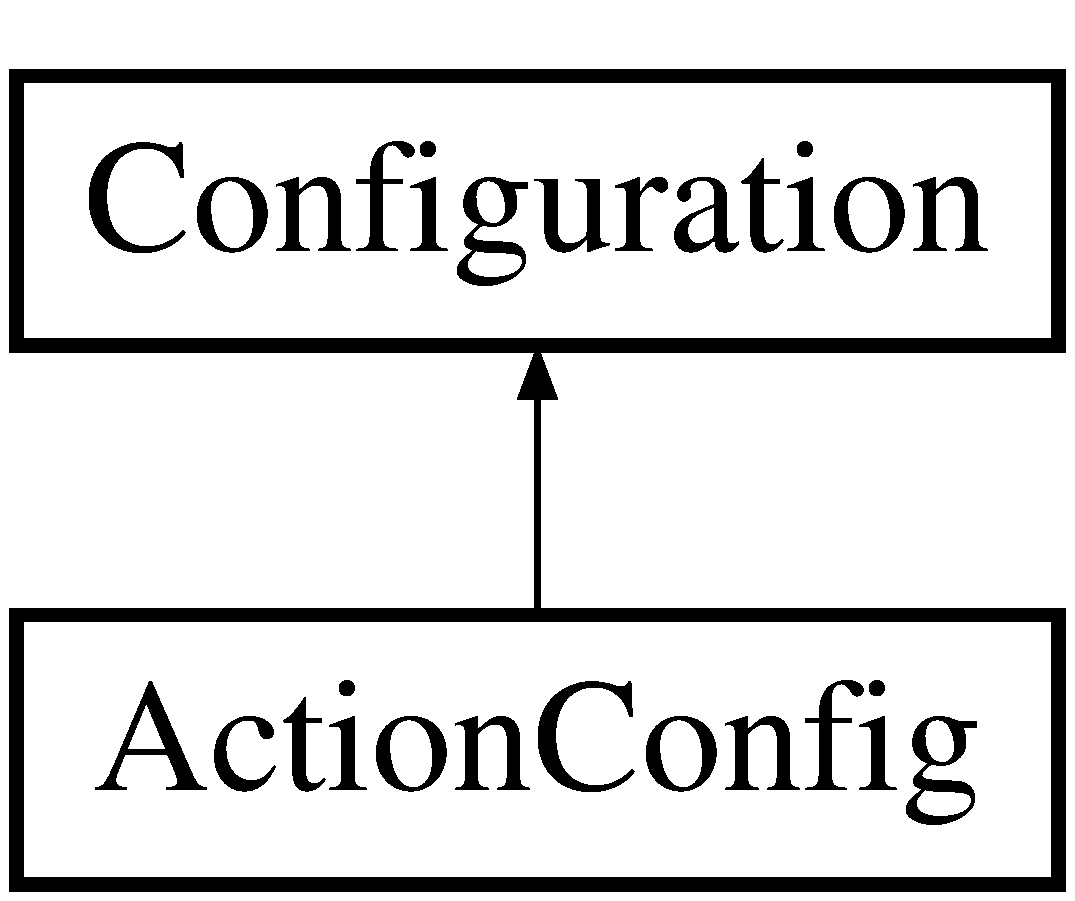
\includegraphics[height=2.000000cm]{classActionConfig}
\end{center}
\end{figure}
\subsection*{Public Member Functions}
\begin{DoxyCompactItemize}
\item 
bool \hyperlink{classActionConfig_a822bda3a3ae83a30d6e7d297ca80c451}{do\-Comparison} (\hyperlink{classConfiguration}{Configuration} $\ast$c)
\begin{DoxyCompactList}\small\item\em Accept a configuration to do a comparision on. \end{DoxyCompactList}\item 
bool \hyperlink{classActionConfig_adbf2b04b558792a6fcfef7a52d16411c}{Compare} (\hyperlink{classConfiguration}{Configuration} $\ast$c)
\begin{DoxyCompactList}\small\item\em Do the comparison on the configuration. \end{DoxyCompactList}\end{DoxyCompactItemize}
\subsection*{Public Attributes}
\begin{DoxyCompactItemize}
\item 
\hypertarget{classActionConfig_ac633fa67b421cf574fd42f01179c5d49}{float {\bfseries a1}}\label{classActionConfig_ac633fa67b421cf574fd42f01179c5d49}

\item 
float \hyperlink{classActionConfig_a6e64f27b8bc62c437d43d45a0bc201c8}{a2}
\end{DoxyCompactItemize}


\subsection{Detailed Description}
\hyperlink{classAction}{Action} configuration class to hold change in joint variables used with the \hyperlink{classAction}{Action} class. 

\subsection{Member Function Documentation}
\hypertarget{classActionConfig_adbf2b04b558792a6fcfef7a52d16411c}{\index{Action\-Config@{Action\-Config}!Compare@{Compare}}
\index{Compare@{Compare}!ActionConfig@{Action\-Config}}
\subsubsection[{Compare}]{\setlength{\rightskip}{0pt plus 5cm}bool Action\-Config\-::\-Compare (
\begin{DoxyParamCaption}
\item[{{\bf Configuration} $\ast$}]{c}
\end{DoxyParamCaption}
)\hspace{0.3cm}{\ttfamily [virtual]}}}\label{classActionConfig_adbf2b04b558792a6fcfef7a52d16411c}


Do the comparison on the configuration. 


\begin{DoxyParams}[1]{Parameters}
\mbox{\tt in}  & {\em c} & The configuration to compare. \\
\hline
\end{DoxyParams}
\begin{DoxyReturn}{Returns}
If the configuration passed in is equal to this one. 
\end{DoxyReturn}


Implements \hyperlink{classConfiguration_a82f926a9b9ea439862089f1d6c06b3e0}{Configuration}.

\hypertarget{classActionConfig_a822bda3a3ae83a30d6e7d297ca80c451}{\index{Action\-Config@{Action\-Config}!do\-Comparison@{do\-Comparison}}
\index{do\-Comparison@{do\-Comparison}!ActionConfig@{Action\-Config}}
\subsubsection[{do\-Comparison}]{\setlength{\rightskip}{0pt plus 5cm}bool Action\-Config\-::do\-Comparison (
\begin{DoxyParamCaption}
\item[{{\bf Configuration} $\ast$}]{c}
\end{DoxyParamCaption}
)\hspace{0.3cm}{\ttfamily [virtual]}}}\label{classActionConfig_a822bda3a3ae83a30d6e7d297ca80c451}


Accept a configuration to do a comparision on. 


\begin{DoxyParams}[1]{Parameters}
\mbox{\tt in}  & {\em c} & The configuration to compare with this one. \\
\hline
\end{DoxyParams}
\begin{DoxyReturn}{Returns}
If the comparison was sucessful. 
\end{DoxyReturn}


Implements \hyperlink{classConfiguration_a0bc4a5154c2836cc8976049810b35548}{Configuration}.



\subsection{Member Data Documentation}
\hypertarget{classActionConfig_a6e64f27b8bc62c437d43d45a0bc201c8}{\index{Action\-Config@{Action\-Config}!a2@{a2}}
\index{a2@{a2}!ActionConfig@{Action\-Config}}
\subsubsection[{a2}]{\setlength{\rightskip}{0pt plus 5cm}float Action\-Config\-::a2}}\label{classActionConfig_a6e64f27b8bc62c437d43d45a0bc201c8}
\hyperlink{classAction}{Action} for each joint. 

The documentation for this class was generated from the following file\-:\begin{DoxyCompactItemize}
\item 
crawler.\-h\end{DoxyCompactItemize}

\hypertarget{classActionSet}{\section{Action\-Set Class Reference}
\label{classActionSet}\index{Action\-Set@{Action\-Set}}
}


\hyperlink{classActionSet}{Action\-Set} class.  




{\ttfamily \#include $<$rl-\/lib\-\_\-state.\-h$>$}

\subsection*{Public Member Functions}
\begin{DoxyCompactItemize}
\item 
\hyperlink{classActionSet_af1a45dd53e14b66eabf1a4e77df51c81}{Action\-Set} ()
\begin{DoxyCompactList}\small\item\em Default constructor for the set. \end{DoxyCompactList}\item 
\hyperlink{classActionSet_a4b5f488670ee207dbb3aac3f92e83bd3}{Action\-Set} (int n)
\begin{DoxyCompactList}\small\item\em Constructor for the set with known size. \end{DoxyCompactList}\item 
\hypertarget{classActionSet_a95eb8d8a76dfdda76cf4cbc67c6e070b}{\hyperlink{classActionSet_a95eb8d8a76dfdda76cf4cbc67c6e070b}{$\sim$\-Action\-Set} ()}\label{classActionSet_a95eb8d8a76dfdda76cf4cbc67c6e070b}

\begin{DoxyCompactList}\small\item\em Default destructor for the set. \end{DoxyCompactList}\item 
void \hyperlink{classActionSet_a2283fd90299aa1b8390c5957164032b8}{push} (\hyperlink{classAction}{Action} a)
\begin{DoxyCompactList}\small\item\em Add \hyperlink{classAction}{Action} to the set. \end{DoxyCompactList}\item 
\hyperlink{classAction}{Action} \hyperlink{classActionSet_a079095c7b16385741f48c1f75bc225ba}{pop} ()
\begin{DoxyCompactList}\small\item\em Remove \hyperlink{classAction}{Action} from the set. \end{DoxyCompactList}\item 
bool \hyperlink{classActionSet_a76b75c1f8ce17b41f3868c3ef845daf6}{is\-Empty} ()
\begin{DoxyCompactList}\small\item\em Are there any objects in the set? \end{DoxyCompactList}\item 
int \hyperlink{classActionSet_aa41e9f5b446070bf5b57d9d314b3960c}{size} ()
\begin{DoxyCompactList}\small\item\em How many Actions are in this set? \end{DoxyCompactList}\item 
\hypertarget{classActionSet_aee6a3a79570dd883dafdd66285f2eb39}{\hyperlink{classActionSetIter}{Action\-Set\-Iter} $\ast$ \hyperlink{classActionSet_aee6a3a79570dd883dafdd66285f2eb39}{create\-Iter} () const }\label{classActionSet_aee6a3a79570dd883dafdd66285f2eb39}

\begin{DoxyCompactList}\small\item\em Create iterator for set. \end{DoxyCompactList}\end{DoxyCompactItemize}
\subsection*{Friends}
\begin{DoxyCompactItemize}
\item 
\hypertarget{classActionSet_aadd7d34449f2080eeb1259cf3ce0c141}{class \hyperlink{classActionSet_aadd7d34449f2080eeb1259cf3ce0c141}{Action\-Set\-Iter}}\label{classActionSet_aadd7d34449f2080eeb1259cf3ce0c141}

\begin{DoxyCompactList}\small\item\em Declare iterator class as friend. \end{DoxyCompactList}\end{DoxyCompactItemize}


\subsection{Detailed Description}
\hyperlink{classActionSet}{Action\-Set} class. 

This is an aggregate class for containing a set of \hyperlink{classAction}{Action} objects. 

\subsection{Constructor \& Destructor Documentation}
\hypertarget{classActionSet_af1a45dd53e14b66eabf1a4e77df51c81}{\index{Action\-Set@{Action\-Set}!Action\-Set@{Action\-Set}}
\index{Action\-Set@{Action\-Set}!ActionSet@{Action\-Set}}
\subsubsection[{Action\-Set}]{\setlength{\rightskip}{0pt plus 5cm}Action\-Set\-::\-Action\-Set (
\begin{DoxyParamCaption}
{}
\end{DoxyParamCaption}
)}}\label{classActionSet_af1a45dd53e14b66eabf1a4e77df51c81}


Default constructor for the set. 

$\ast$$\ast$$\ast$ \hyperlink{classActionSet}{Action\-Set} class. $\ast$$\ast$$\ast$///

Default constructor for the set. \hypertarget{classActionSet_a4b5f488670ee207dbb3aac3f92e83bd3}{\index{Action\-Set@{Action\-Set}!Action\-Set@{Action\-Set}}
\index{Action\-Set@{Action\-Set}!ActionSet@{Action\-Set}}
\subsubsection[{Action\-Set}]{\setlength{\rightskip}{0pt plus 5cm}Action\-Set\-::\-Action\-Set (
\begin{DoxyParamCaption}
\item[{int}]{n}
\end{DoxyParamCaption}
)}}\label{classActionSet_a4b5f488670ee207dbb3aac3f92e83bd3}


Constructor for the set with known size. 


\begin{DoxyParams}[1]{Parameters}
\mbox{\tt in}  & {\em n} & The number of actions in the set. \\
\hline
\end{DoxyParams}


\subsection{Member Function Documentation}
\hypertarget{classActionSet_a76b75c1f8ce17b41f3868c3ef845daf6}{\index{Action\-Set@{Action\-Set}!is\-Empty@{is\-Empty}}
\index{is\-Empty@{is\-Empty}!ActionSet@{Action\-Set}}
\subsubsection[{is\-Empty}]{\setlength{\rightskip}{0pt plus 5cm}bool Action\-Set\-::is\-Empty (
\begin{DoxyParamCaption}
{}
\end{DoxyParamCaption}
)}}\label{classActionSet_a76b75c1f8ce17b41f3868c3ef845daf6}


Are there any objects in the set? 

\begin{DoxyReturn}{Returns}
Returns true if there is anything in the set. 
\end{DoxyReturn}
\hypertarget{classActionSet_a079095c7b16385741f48c1f75bc225ba}{\index{Action\-Set@{Action\-Set}!pop@{pop}}
\index{pop@{pop}!ActionSet@{Action\-Set}}
\subsubsection[{pop}]{\setlength{\rightskip}{0pt plus 5cm}{\bf Action} Action\-Set\-::pop (
\begin{DoxyParamCaption}
{}
\end{DoxyParamCaption}
)}}\label{classActionSet_a079095c7b16385741f48c1f75bc225ba}


Remove \hyperlink{classAction}{Action} from the set. 

\begin{DoxyReturn}{Returns}
\hyperlink{classAction}{Action} object removed from the set. 
\end{DoxyReturn}
\hypertarget{classActionSet_a2283fd90299aa1b8390c5957164032b8}{\index{Action\-Set@{Action\-Set}!push@{push}}
\index{push@{push}!ActionSet@{Action\-Set}}
\subsubsection[{push}]{\setlength{\rightskip}{0pt plus 5cm}void Action\-Set\-::push (
\begin{DoxyParamCaption}
\item[{{\bf Action}}]{a}
\end{DoxyParamCaption}
)}}\label{classActionSet_a2283fd90299aa1b8390c5957164032b8}


Add \hyperlink{classAction}{Action} to the set. 


\begin{DoxyParams}[1]{Parameters}
\mbox{\tt in}  & {\em a} & \hyperlink{classAction}{Action} to be added to the set. \\
\hline
\end{DoxyParams}
\hypertarget{classActionSet_aa41e9f5b446070bf5b57d9d314b3960c}{\index{Action\-Set@{Action\-Set}!size@{size}}
\index{size@{size}!ActionSet@{Action\-Set}}
\subsubsection[{size}]{\setlength{\rightskip}{0pt plus 5cm}int Action\-Set\-::size (
\begin{DoxyParamCaption}
{}
\end{DoxyParamCaption}
)}}\label{classActionSet_aa41e9f5b446070bf5b57d9d314b3960c}


How many Actions are in this set? 

\begin{DoxyReturn}{Returns}
Returns the number of Actions in the set. 
\end{DoxyReturn}


The documentation for this class was generated from the following files\-:\begin{DoxyCompactItemize}
\item 
rl-\/lib\-\_\-state.\-h\item 
rl-\/lib\-\_\-state.\-cpp\end{DoxyCompactItemize}

\hypertarget{classActionSetIter}{\section{Action\-Set\-Iter Class Reference}
\label{classActionSetIter}\index{Action\-Set\-Iter@{Action\-Set\-Iter}}
}


Iterator class for \hyperlink{classActionSet}{Action\-Set}.  




{\ttfamily \#include $<$rl-\/lib\-\_\-state.\-h$>$}

\subsection*{Public Member Functions}
\begin{DoxyCompactItemize}
\item 
\hyperlink{classActionSetIter_a7e0b7dae76dd05e57de36d17ea410edb}{Action\-Set\-Iter} (const \hyperlink{classActionSet}{Action\-Set} $\ast$as)
\begin{DoxyCompactList}\small\item\em Constructor taking \hyperlink{classActionSet}{Action\-Set} associated with iterator. \end{DoxyCompactList}\item 
\hypertarget{classActionSetIter_aa0f694797b7003987ce46624ad756b14}{void \hyperlink{classActionSetIter_aa0f694797b7003987ce46624ad756b14}{first} ()}\label{classActionSetIter_aa0f694797b7003987ce46624ad756b14}

\begin{DoxyCompactList}\small\item\em Set the iterator to the first element of the set. \end{DoxyCompactList}\item 
\hypertarget{classActionSetIter_a5aab0600528fb3af00d1b3b0d8cfd673}{void \hyperlink{classActionSetIter_a5aab0600528fb3af00d1b3b0d8cfd673}{next} ()}\label{classActionSetIter_a5aab0600528fb3af00d1b3b0d8cfd673}

\begin{DoxyCompactList}\small\item\em Increment the iterator. \end{DoxyCompactList}\item 
\hypertarget{classActionSetIter_a7df2acfbd850b7e36c2a9a5884fb6d3a}{bool \hyperlink{classActionSetIter_a7df2acfbd850b7e36c2a9a5884fb6d3a}{is\-Done} ()}\label{classActionSetIter_a7df2acfbd850b7e36c2a9a5884fb6d3a}

\begin{DoxyCompactList}\small\item\em Check to see if we are at the last element. \end{DoxyCompactList}\item 
\hypertarget{classActionSetIter_abc71e0880f2f33824658de4a73598683}{\hyperlink{classAction}{Action} \hyperlink{classActionSetIter_abc71e0880f2f33824658de4a73598683}{operator$\ast$} ()}\label{classActionSetIter_abc71e0880f2f33824658de4a73598683}

\begin{DoxyCompactList}\small\item\em Dereference operator. \end{DoxyCompactList}\item 
\hypertarget{classActionSetIter_af824ed984a83a78e1affdbe89f25a43b}{\hyperlink{classAction}{Action} $\ast$ \hyperlink{classActionSetIter_af824ed984a83a78e1affdbe89f25a43b}{operator-\/$>$} () const }\label{classActionSetIter_af824ed984a83a78e1affdbe89f25a43b}

\begin{DoxyCompactList}\small\item\em Arrow operator. \end{DoxyCompactList}\end{DoxyCompactItemize}


\subsection{Detailed Description}
Iterator class for \hyperlink{classActionSet}{Action\-Set}. 

\subsection{Constructor \& Destructor Documentation}
\hypertarget{classActionSetIter_a7e0b7dae76dd05e57de36d17ea410edb}{\index{Action\-Set\-Iter@{Action\-Set\-Iter}!Action\-Set\-Iter@{Action\-Set\-Iter}}
\index{Action\-Set\-Iter@{Action\-Set\-Iter}!ActionSetIter@{Action\-Set\-Iter}}
\subsubsection[{Action\-Set\-Iter}]{\setlength{\rightskip}{0pt plus 5cm}Action\-Set\-Iter\-::\-Action\-Set\-Iter (
\begin{DoxyParamCaption}
\item[{const {\bf Action\-Set} $\ast$}]{as}
\end{DoxyParamCaption}
)}}\label{classActionSetIter_a7e0b7dae76dd05e57de36d17ea410edb}


Constructor taking \hyperlink{classActionSet}{Action\-Set} associated with iterator. 

$\ast$$\ast$$\ast$ Iterator class for \hyperlink{classActionSet}{Action\-Set}. $\ast$$\ast$$\ast$///


\begin{DoxyParams}[1]{Parameters}
\mbox{\tt in}  & {\em as} & Pointer to the \hyperlink{classActionSet}{Action\-Set} for this iterator.\\
\hline
\end{DoxyParams}
Constructor taking \hyperlink{classActionSet}{Action\-Set} associated with iterator. 
\begin{DoxyParams}[1]{Parameters}
\mbox{\tt in}  & {\em as} & Pointer to the \hyperlink{classActionSet}{Action\-Set} for this iterator. \\
\hline
\end{DoxyParams}


The documentation for this class was generated from the following files\-:\begin{DoxyCompactItemize}
\item 
rl-\/lib\-\_\-state.\-h\item 
rl-\/lib\-\_\-state.\-cpp\end{DoxyCompactItemize}

\hypertarget{classArm}{\section{Arm Class Reference}
\label{classArm}\index{Arm@{Arm}}
}


\hyperlink{classArm}{Arm} class for assigning angles to the crawler arm.  




{\ttfamily \#include $<$crawler.\-h$>$}

\subsection*{Public Member Functions}
\begin{DoxyCompactItemize}
\item 
\hyperlink{classArm_a920d0f828c6e76188827cf0c073963de}{Arm} ()
\begin{DoxyCompactList}\small\item\em Default constructor. \end{DoxyCompactList}\item 
void \hyperlink{classArm_a51bf7b1e2395c7437dd307ea689bd63e}{set\-Joint\-Angle} (int joint, float angle)
\begin{DoxyCompactList}\small\item\em Sets joint angles for the arm class. \end{DoxyCompactList}\item 
void \hyperlink{classArm_a3420d04cfe246e50b7d06dfc438184b0}{set\-Joint\-Config} (float angle1, float angle2)
\begin{DoxyCompactList}\small\item\em Sets both joint angles for the arm class. \end{DoxyCompactList}\item 
float \hyperlink{classArm_ac02320e3e99d6ff5c216f991b3540f5d}{get\-Joint\-Angle} (int joint)
\begin{DoxyCompactList}\small\item\em Gets joint angles for the arm class. \end{DoxyCompactList}\item 
float \hyperlink{classArm_a27305db80b3780b83162d63a19693d0b}{get\-Joint\-Angle\-Calibrated} (int joint)
\begin{DoxyCompactList}\small\item\em Gets joint angles for the arm class to be sent to the servos. \end{DoxyCompactList}\item 
int \hyperlink{classArm_a3be1d9132b03b8d8ea120271f699fd5a}{get\-Joint\-Pin} (int joint)
\begin{DoxyCompactList}\small\item\em Gets the Arduino pin assignment for that joint. \end{DoxyCompactList}\end{DoxyCompactItemize}


\subsection{Detailed Description}
\hyperlink{classArm}{Arm} class for assigning angles to the crawler arm. 

This class is for assigning arm values but itself does not command the hardware. The calibrated values must be taken from it and given to the servo driver. 

\subsection{Constructor \& Destructor Documentation}
\hypertarget{classArm_a920d0f828c6e76188827cf0c073963de}{\index{Arm@{Arm}!Arm@{Arm}}
\index{Arm@{Arm}!Arm@{Arm}}
\subsubsection[{Arm}]{\setlength{\rightskip}{0pt plus 5cm}Arm\-::\-Arm (
\begin{DoxyParamCaption}
{}
\end{DoxyParamCaption}
)}}\label{classArm_a920d0f828c6e76188827cf0c073963de}


Default constructor. 

$\ast$$\ast$$\ast$ \hyperlink{classArm}{Arm} Class $\ast$$\ast$$\ast$/// 

\subsection{Member Function Documentation}
\hypertarget{classArm_ac02320e3e99d6ff5c216f991b3540f5d}{\index{Arm@{Arm}!get\-Joint\-Angle@{get\-Joint\-Angle}}
\index{get\-Joint\-Angle@{get\-Joint\-Angle}!Arm@{Arm}}
\subsubsection[{get\-Joint\-Angle}]{\setlength{\rightskip}{0pt plus 5cm}float Arm\-::get\-Joint\-Angle (
\begin{DoxyParamCaption}
\item[{int}]{joint}
\end{DoxyParamCaption}
)}}\label{classArm_ac02320e3e99d6ff5c216f991b3540f5d}


Gets joint angles for the arm class. 


\begin{DoxyParams}[1]{Parameters}
\mbox{\tt in}  & {\em joint} & The joint to get the angle for. \\
\hline
\end{DoxyParams}
\begin{DoxyReturn}{Returns}
The angle for the given joint in degrees. 
\end{DoxyReturn}
\hypertarget{classArm_a27305db80b3780b83162d63a19693d0b}{\index{Arm@{Arm}!get\-Joint\-Angle\-Calibrated@{get\-Joint\-Angle\-Calibrated}}
\index{get\-Joint\-Angle\-Calibrated@{get\-Joint\-Angle\-Calibrated}!Arm@{Arm}}
\subsubsection[{get\-Joint\-Angle\-Calibrated}]{\setlength{\rightskip}{0pt plus 5cm}float Arm\-::get\-Joint\-Angle\-Calibrated (
\begin{DoxyParamCaption}
\item[{int}]{joint}
\end{DoxyParamCaption}
)}}\label{classArm_a27305db80b3780b83162d63a19693d0b}


Gets joint angles for the arm class to be sent to the servos. 

Takes into account any calibration parameters needed for correct angle mapping.


\begin{DoxyParams}[1]{Parameters}
\mbox{\tt in}  & {\em joint} & The joint to get the angle for. \\
\hline
\end{DoxyParams}
\begin{DoxyReturn}{Returns}
The angle for the given joint in degrees. 
\end{DoxyReturn}
\hypertarget{classArm_a3be1d9132b03b8d8ea120271f699fd5a}{\index{Arm@{Arm}!get\-Joint\-Pin@{get\-Joint\-Pin}}
\index{get\-Joint\-Pin@{get\-Joint\-Pin}!Arm@{Arm}}
\subsubsection[{get\-Joint\-Pin}]{\setlength{\rightskip}{0pt plus 5cm}int Arm\-::get\-Joint\-Pin (
\begin{DoxyParamCaption}
\item[{int}]{joint}
\end{DoxyParamCaption}
)}}\label{classArm_a3be1d9132b03b8d8ea120271f699fd5a}


Gets the Arduino pin assignment for that joint. 


\begin{DoxyParams}[1]{Parameters}
\mbox{\tt in}  & {\em joint} & The joint to get the pin number for. \\
\hline
\end{DoxyParams}
\begin{DoxyReturn}{Returns}
The pin number for that joint. 
\end{DoxyReturn}
\hypertarget{classArm_a51bf7b1e2395c7437dd307ea689bd63e}{\index{Arm@{Arm}!set\-Joint\-Angle@{set\-Joint\-Angle}}
\index{set\-Joint\-Angle@{set\-Joint\-Angle}!Arm@{Arm}}
\subsubsection[{set\-Joint\-Angle}]{\setlength{\rightskip}{0pt plus 5cm}void Arm\-::set\-Joint\-Angle (
\begin{DoxyParamCaption}
\item[{int}]{joint, }
\item[{float}]{angle}
\end{DoxyParamCaption}
)}}\label{classArm_a51bf7b1e2395c7437dd307ea689bd63e}


Sets joint angles for the arm class. 


\begin{DoxyParams}[1]{Parameters}
\mbox{\tt in}  & {\em joint} & Which joint in the chain to be commanded. \\
\hline
\mbox{\tt in}  & {\em angle} & The angle to which the joint will be commanded. \\
\hline
\end{DoxyParams}
\hypertarget{classArm_a3420d04cfe246e50b7d06dfc438184b0}{\index{Arm@{Arm}!set\-Joint\-Config@{set\-Joint\-Config}}
\index{set\-Joint\-Config@{set\-Joint\-Config}!Arm@{Arm}}
\subsubsection[{set\-Joint\-Config}]{\setlength{\rightskip}{0pt plus 5cm}void Arm\-::set\-Joint\-Config (
\begin{DoxyParamCaption}
\item[{float}]{angle1, }
\item[{float}]{angle2}
\end{DoxyParamCaption}
)}}\label{classArm_a3420d04cfe246e50b7d06dfc438184b0}


Sets both joint angles for the arm class. 


\begin{DoxyParams}[1]{Parameters}
\mbox{\tt in}  & {\em angle1} & Angle of the first joint, J1. \\
\hline
\mbox{\tt in}  & {\em angle2} & Angle of the second joint, J2. \\
\hline
\end{DoxyParams}


The documentation for this class was generated from the following files\-:\begin{DoxyCompactItemize}
\item 
crawler.\-h\item 
crawler.\-cpp\end{DoxyCompactItemize}

\hypertarget{classArmConfig}{\section{Arm\-Config Class Reference}
\label{classArmConfig}\index{Arm\-Config@{Arm\-Config}}
}


\hyperlink{classArm}{Arm} configuration class to hold joint variables used with the \hyperlink{classState}{State} class.  




{\ttfamily \#include $<$crawler.\-h$>$}

Inheritance diagram for Arm\-Config\-:\begin{figure}[H]
\begin{center}
\leavevmode
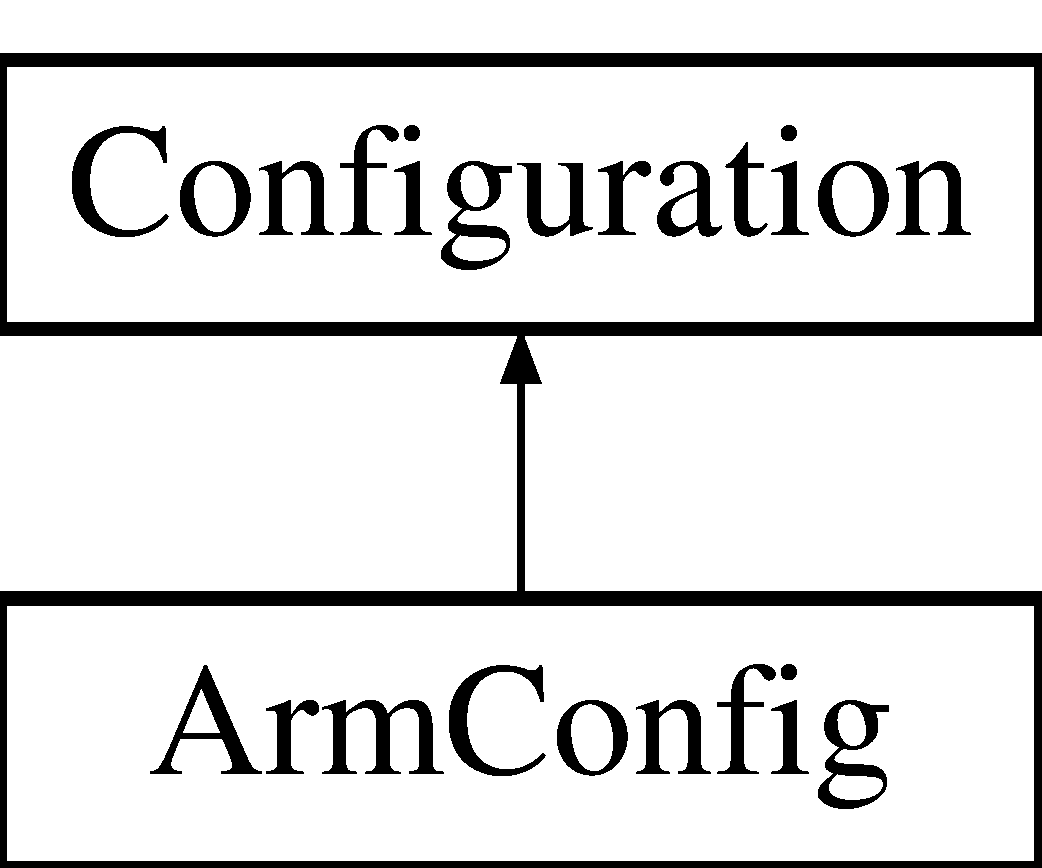
\includegraphics[height=2.000000cm]{classArmConfig}
\end{center}
\end{figure}
\subsection*{Public Member Functions}
\begin{DoxyCompactItemize}
\item 
bool \hyperlink{classArmConfig_a9c88c588472e0c18024d4a6c30f1f531}{do\-Comparison} (\hyperlink{classConfiguration}{Configuration} $\ast$c)
\begin{DoxyCompactList}\small\item\em Accept a configuration to do a comparision on. \end{DoxyCompactList}\item 
bool \hyperlink{classArmConfig_af97e33e4a0b4faaf611737e375e15e23}{Compare} (\hyperlink{classConfiguration}{Configuration} $\ast$c)
\begin{DoxyCompactList}\small\item\em Do the comparison on the configuration. \end{DoxyCompactList}\item 
bool \hyperlink{classArmConfig_a91931a29109e8b018d1c600c462fb95f}{Compare} (\hyperlink{classArmConfig}{Arm\-Config} $\ast$c)
\begin{DoxyCompactList}\small\item\em Do the comparison on the arm configuration. \end{DoxyCompactList}\end{DoxyCompactItemize}
\subsection*{Public Attributes}
\begin{DoxyCompactItemize}
\item 
\hypertarget{classArmConfig_a2fb3ed359d34f8a61707dc15a791f2fc}{float {\bfseries angle1}}\label{classArmConfig_a2fb3ed359d34f8a61707dc15a791f2fc}

\item 
float \hyperlink{classArmConfig_a8675cabacd6a5a75d9dd21696b14f645}{angle2}
\end{DoxyCompactItemize}


\subsection{Detailed Description}
\hyperlink{classArm}{Arm} configuration class to hold joint variables used with the \hyperlink{classState}{State} class. 

\subsection{Member Function Documentation}
\hypertarget{classArmConfig_af97e33e4a0b4faaf611737e375e15e23}{\index{Arm\-Config@{Arm\-Config}!Compare@{Compare}}
\index{Compare@{Compare}!ArmConfig@{Arm\-Config}}
\subsubsection[{Compare}]{\setlength{\rightskip}{0pt plus 5cm}bool Arm\-Config\-::\-Compare (
\begin{DoxyParamCaption}
\item[{{\bf Configuration} $\ast$}]{c}
\end{DoxyParamCaption}
)\hspace{0.3cm}{\ttfamily [virtual]}}}\label{classArmConfig_af97e33e4a0b4faaf611737e375e15e23}


Do the comparison on the configuration. 

Will return false as the abstract type cannot be compared to the derived type.


\begin{DoxyParams}[1]{Parameters}
\mbox{\tt in}  & {\em c} & The \hyperlink{classConfiguration}{Configuration} to compare. \\
\hline
\end{DoxyParams}
\begin{DoxyReturn}{Returns}
If the configuration passed in is equal to this one. 
\end{DoxyReturn}


Implements \hyperlink{classConfiguration_a82f926a9b9ea439862089f1d6c06b3e0}{Configuration}.

\hypertarget{classArmConfig_a91931a29109e8b018d1c600c462fb95f}{\index{Arm\-Config@{Arm\-Config}!Compare@{Compare}}
\index{Compare@{Compare}!ArmConfig@{Arm\-Config}}
\subsubsection[{Compare}]{\setlength{\rightskip}{0pt plus 5cm}bool Arm\-Config\-::\-Compare (
\begin{DoxyParamCaption}
\item[{{\bf Arm\-Config} $\ast$}]{c}
\end{DoxyParamCaption}
)}}\label{classArmConfig_a91931a29109e8b018d1c600c462fb95f}


Do the comparison on the arm configuration. 


\begin{DoxyParams}[1]{Parameters}
\mbox{\tt in}  & {\em c} & The \hyperlink{classArmConfig}{Arm\-Config} to compare. \\
\hline
\end{DoxyParams}
\begin{DoxyReturn}{Returns}
If the configuration passed in is equal to this one. 
\end{DoxyReturn}
\hypertarget{classArmConfig_a9c88c588472e0c18024d4a6c30f1f531}{\index{Arm\-Config@{Arm\-Config}!do\-Comparison@{do\-Comparison}}
\index{do\-Comparison@{do\-Comparison}!ArmConfig@{Arm\-Config}}
\subsubsection[{do\-Comparison}]{\setlength{\rightskip}{0pt plus 5cm}bool Arm\-Config\-::do\-Comparison (
\begin{DoxyParamCaption}
\item[{{\bf Configuration} $\ast$}]{c}
\end{DoxyParamCaption}
)\hspace{0.3cm}{\ttfamily [virtual]}}}\label{classArmConfig_a9c88c588472e0c18024d4a6c30f1f531}


Accept a configuration to do a comparision on. 

$\ast$$\ast$$\ast$ \hyperlink{classArmConfig}{Arm\-Config} Class $\ast$$\ast$$\ast$///


\begin{DoxyParams}[1]{Parameters}
\mbox{\tt in}  & {\em c} & The configuration to compare with this one. \\
\hline
\end{DoxyParams}
\begin{DoxyReturn}{Returns}
If the comparison was sucessful. 
\end{DoxyReturn}


Implements \hyperlink{classConfiguration_a0bc4a5154c2836cc8976049810b35548}{Configuration}.



\subsection{Member Data Documentation}
\hypertarget{classArmConfig_a8675cabacd6a5a75d9dd21696b14f645}{\index{Arm\-Config@{Arm\-Config}!angle2@{angle2}}
\index{angle2@{angle2}!ArmConfig@{Arm\-Config}}
\subsubsection[{angle2}]{\setlength{\rightskip}{0pt plus 5cm}float Arm\-Config\-::angle2}}\label{classArmConfig_a8675cabacd6a5a75d9dd21696b14f645}
Angles for each of the joints. 

The documentation for this class was generated from the following files\-:\begin{DoxyCompactItemize}
\item 
crawler.\-h\item 
crawler.\-cpp\end{DoxyCompactItemize}

\hypertarget{classConfiguration}{\section{Configuration Class Reference}
\label{classConfiguration}\index{Configuration@{Configuration}}
}


\hyperlink{classConfiguration}{Configuration} class.  




{\ttfamily \#include $<$rl-\/lib\-\_\-state.\-h$>$}

Inheritance diagram for Configuration\-:\begin{figure}[H]
\begin{center}
\leavevmode
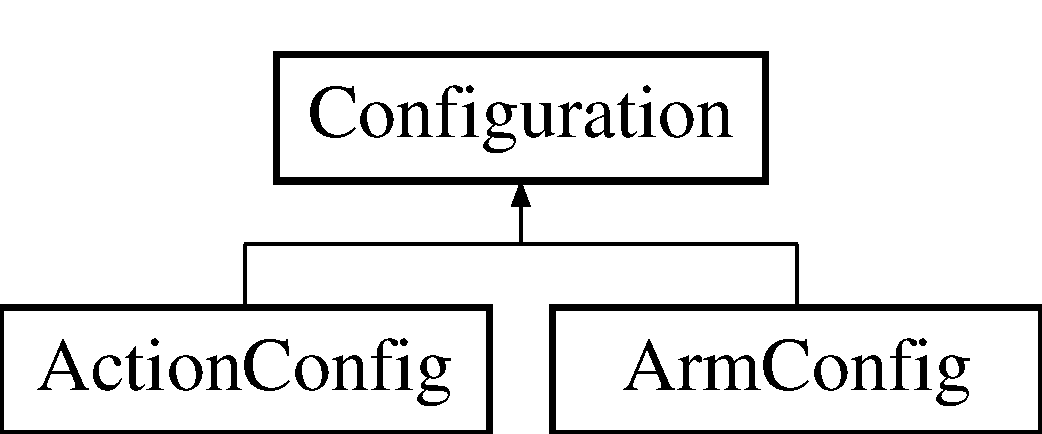
\includegraphics[height=2.000000cm]{classConfiguration}
\end{center}
\end{figure}
\subsection*{Public Member Functions}
\begin{DoxyCompactItemize}
\item 
virtual bool \hyperlink{classConfiguration_a0bc4a5154c2836cc8976049810b35548}{do\-Comparison} (\hyperlink{classConfiguration}{Configuration} $\ast$c)=0
\begin{DoxyCompactList}\small\item\em Accept a configuration to do a comparision on. \end{DoxyCompactList}\item 
virtual bool \hyperlink{classConfiguration_a82f926a9b9ea439862089f1d6c06b3e0}{Compare} (\hyperlink{classConfiguration}{Configuration} $\ast$c)=0
\begin{DoxyCompactList}\small\item\em Do the comparison on the configuration. \end{DoxyCompactList}\end{DoxyCompactItemize}


\subsection{Detailed Description}
\hyperlink{classConfiguration}{Configuration} class. 

This class is for creating system state or configurations that the system would actually be in. For example, for a arm, it might be a set of joint angles. 

\subsection{Member Function Documentation}
\hypertarget{classConfiguration_a82f926a9b9ea439862089f1d6c06b3e0}{\index{Configuration@{Configuration}!Compare@{Compare}}
\index{Compare@{Compare}!Configuration@{Configuration}}
\subsubsection[{Compare}]{\setlength{\rightskip}{0pt plus 5cm}virtual bool Configuration\-::\-Compare (
\begin{DoxyParamCaption}
\item[{{\bf Configuration} $\ast$}]{c}
\end{DoxyParamCaption}
)\hspace{0.3cm}{\ttfamily [pure virtual]}}}\label{classConfiguration_a82f926a9b9ea439862089f1d6c06b3e0}


Do the comparison on the configuration. 


\begin{DoxyParams}[1]{Parameters}
\mbox{\tt in}  & {\em c} & The configuration to compare. \\
\hline
\end{DoxyParams}
\begin{DoxyReturn}{Returns}
If the configuration passed in is equal to this one. 
\end{DoxyReturn}


Implemented in \hyperlink{classActionConfig_adbf2b04b558792a6fcfef7a52d16411c}{Action\-Config}, and \hyperlink{classArmConfig_af97e33e4a0b4faaf611737e375e15e23}{Arm\-Config}.

\hypertarget{classConfiguration_a0bc4a5154c2836cc8976049810b35548}{\index{Configuration@{Configuration}!do\-Comparison@{do\-Comparison}}
\index{do\-Comparison@{do\-Comparison}!Configuration@{Configuration}}
\subsubsection[{do\-Comparison}]{\setlength{\rightskip}{0pt plus 5cm}virtual bool Configuration\-::do\-Comparison (
\begin{DoxyParamCaption}
\item[{{\bf Configuration} $\ast$}]{c}
\end{DoxyParamCaption}
)\hspace{0.3cm}{\ttfamily [pure virtual]}}}\label{classConfiguration_a0bc4a5154c2836cc8976049810b35548}


Accept a configuration to do a comparision on. 


\begin{DoxyParams}[1]{Parameters}
\mbox{\tt in}  & {\em c} & The configuration to compare with this one. \\
\hline
\end{DoxyParams}
\begin{DoxyReturn}{Returns}
If the comparison was sucessful. 
\end{DoxyReturn}


Implemented in \hyperlink{classActionConfig_a822bda3a3ae83a30d6e7d297ca80c451}{Action\-Config}, and \hyperlink{classArmConfig_a9c88c588472e0c18024d4a6c30f1f531}{Arm\-Config}.



The documentation for this class was generated from the following file\-:\begin{DoxyCompactItemize}
\item 
rl-\/lib\-\_\-state.\-h\end{DoxyCompactItemize}

\hypertarget{classConfigurationSet}{\section{Configuration\-Set Class Reference}
\label{classConfigurationSet}\index{Configuration\-Set@{Configuration\-Set}}
}


\hyperlink{classConfigurationSet}{Configuration\-Set} class.  




{\ttfamily \#include $<$rl-\/lib\-\_\-state.\-h$>$}

\subsection*{Public Member Functions}
\begin{DoxyCompactItemize}
\item 
\hyperlink{classConfigurationSet_a999e0eafae43cc9eac9b2ece1a808d1c}{Configuration\-Set} ()
\begin{DoxyCompactList}\small\item\em Default constructor for the set. \end{DoxyCompactList}\item 
\hyperlink{classConfigurationSet_aa30585ab5b48d3aec5219d8ecf6decec}{Configuration\-Set} (int n)
\begin{DoxyCompactList}\small\item\em Constructor for the set with known size. \end{DoxyCompactList}\item 
void \hyperlink{classConfigurationSet_a964dd92bef46df4e2b6f8c93ed776e99}{push} (\hyperlink{classConfiguration}{Configuration} $\ast$c)
\begin{DoxyCompactList}\small\item\em Add \hyperlink{classConfiguration}{Configuration} to the set. \end{DoxyCompactList}\item 
\hyperlink{classConfiguration}{Configuration} $\ast$ \hyperlink{classConfigurationSet_a85f2cc23e93e3736edadce7a541b200c}{pop} ()
\begin{DoxyCompactList}\small\item\em Remove \hyperlink{classConfiguration}{Configuration} from the set. \end{DoxyCompactList}\item 
bool \hyperlink{classConfigurationSet_a31e520d14bff315040b43b0da7d050fe}{is\-Empty} ()
\begin{DoxyCompactList}\small\item\em Are there any objects in the set? \end{DoxyCompactList}\item 
int \hyperlink{classConfigurationSet_a0fdde488f125fc12bf8267c39d8bf9c2}{size} ()
\begin{DoxyCompactList}\small\item\em How many Configurations are in this set? \end{DoxyCompactList}\end{DoxyCompactItemize}


\subsection{Detailed Description}
\hyperlink{classConfigurationSet}{Configuration\-Set} class. 

This is an aggregate class for containing a set of \hyperlink{classConfiguration}{Configuration} objects. 

\subsection{Constructor \& Destructor Documentation}
\hypertarget{classConfigurationSet_a999e0eafae43cc9eac9b2ece1a808d1c}{\index{Configuration\-Set@{Configuration\-Set}!Configuration\-Set@{Configuration\-Set}}
\index{Configuration\-Set@{Configuration\-Set}!ConfigurationSet@{Configuration\-Set}}
\subsubsection[{Configuration\-Set}]{\setlength{\rightskip}{0pt plus 5cm}Configuration\-Set\-::\-Configuration\-Set (
\begin{DoxyParamCaption}
{}
\end{DoxyParamCaption}
)}}\label{classConfigurationSet_a999e0eafae43cc9eac9b2ece1a808d1c}


Default constructor for the set. 

$\ast$$\ast$$\ast$ \hyperlink{classConfigurationSet}{Configuration\-Set} $\ast$$\ast$$\ast$///

Default constructor for the set. \hypertarget{classConfigurationSet_aa30585ab5b48d3aec5219d8ecf6decec}{\index{Configuration\-Set@{Configuration\-Set}!Configuration\-Set@{Configuration\-Set}}
\index{Configuration\-Set@{Configuration\-Set}!ConfigurationSet@{Configuration\-Set}}
\subsubsection[{Configuration\-Set}]{\setlength{\rightskip}{0pt plus 5cm}Configuration\-Set\-::\-Configuration\-Set (
\begin{DoxyParamCaption}
\item[{int}]{n}
\end{DoxyParamCaption}
)}}\label{classConfigurationSet_aa30585ab5b48d3aec5219d8ecf6decec}


Constructor for the set with known size. 

Constructor for the set of known size.


\begin{DoxyParams}[1]{Parameters}
\mbox{\tt in}  & {\em n} & The number of configurations in the set. \\
\hline
\end{DoxyParams}


\subsection{Member Function Documentation}
\hypertarget{classConfigurationSet_a31e520d14bff315040b43b0da7d050fe}{\index{Configuration\-Set@{Configuration\-Set}!is\-Empty@{is\-Empty}}
\index{is\-Empty@{is\-Empty}!ConfigurationSet@{Configuration\-Set}}
\subsubsection[{is\-Empty}]{\setlength{\rightskip}{0pt plus 5cm}bool Configuration\-Set\-::is\-Empty (
\begin{DoxyParamCaption}
{}
\end{DoxyParamCaption}
)}}\label{classConfigurationSet_a31e520d14bff315040b43b0da7d050fe}


Are there any objects in the set? 

\begin{DoxyReturn}{Returns}
Returns true if there is anything in the set. 
\end{DoxyReturn}
\hypertarget{classConfigurationSet_a85f2cc23e93e3736edadce7a541b200c}{\index{Configuration\-Set@{Configuration\-Set}!pop@{pop}}
\index{pop@{pop}!ConfigurationSet@{Configuration\-Set}}
\subsubsection[{pop}]{\setlength{\rightskip}{0pt plus 5cm}{\bf Configuration} $\ast$ Configuration\-Set\-::pop (
\begin{DoxyParamCaption}
{}
\end{DoxyParamCaption}
)}}\label{classConfigurationSet_a85f2cc23e93e3736edadce7a541b200c}


Remove \hyperlink{classConfiguration}{Configuration} from the set. 

\begin{DoxyReturn}{Returns}
\hyperlink{classConfiguration}{Configuration} object removed from the set.

Pointer to the \hyperlink{classConfiguration}{Configuration} object removed from the set. 
\end{DoxyReturn}
\hypertarget{classConfigurationSet_a964dd92bef46df4e2b6f8c93ed776e99}{\index{Configuration\-Set@{Configuration\-Set}!push@{push}}
\index{push@{push}!ConfigurationSet@{Configuration\-Set}}
\subsubsection[{push}]{\setlength{\rightskip}{0pt plus 5cm}void Configuration\-Set\-::push (
\begin{DoxyParamCaption}
\item[{{\bf Configuration} $\ast$}]{c}
\end{DoxyParamCaption}
)}}\label{classConfigurationSet_a964dd92bef46df4e2b6f8c93ed776e99}


Add \hyperlink{classConfiguration}{Configuration} to the set. 


\begin{DoxyParams}[1]{Parameters}
\mbox{\tt in}  & {\em c} & \hyperlink{classConfiguration}{Configuration} to be added to the set.\\
\hline
\mbox{\tt in}  & {\em c} & Pointer to the \hyperlink{classConfiguration}{Configuration} to be added to the set. \\
\hline
\end{DoxyParams}
\hypertarget{classConfigurationSet_a0fdde488f125fc12bf8267c39d8bf9c2}{\index{Configuration\-Set@{Configuration\-Set}!size@{size}}
\index{size@{size}!ConfigurationSet@{Configuration\-Set}}
\subsubsection[{size}]{\setlength{\rightskip}{0pt plus 5cm}int Configuration\-Set\-::size (
\begin{DoxyParamCaption}
{}
\end{DoxyParamCaption}
)}}\label{classConfigurationSet_a0fdde488f125fc12bf8267c39d8bf9c2}


How many Configurations are in this set? 

\begin{DoxyReturn}{Returns}
Returns the number of Configurations in the set. 
\end{DoxyReturn}


The documentation for this class was generated from the following files\-:\begin{DoxyCompactItemize}
\item 
rl-\/lib\-\_\-state.\-h\item 
rl-\/lib\-\_\-state.\-cpp\end{DoxyCompactItemize}

\hypertarget{classCrawlerFactory}{\section{Crawler\-Factory Class Reference}
\label{classCrawlerFactory}\index{Crawler\-Factory@{Crawler\-Factory}}
}


Factory class for constructing the state space for the crawler class.  




{\ttfamily \#include $<$crawler.\-h$>$}

Inheritance diagram for Crawler\-Factory\-:\begin{figure}[H]
\begin{center}
\leavevmode
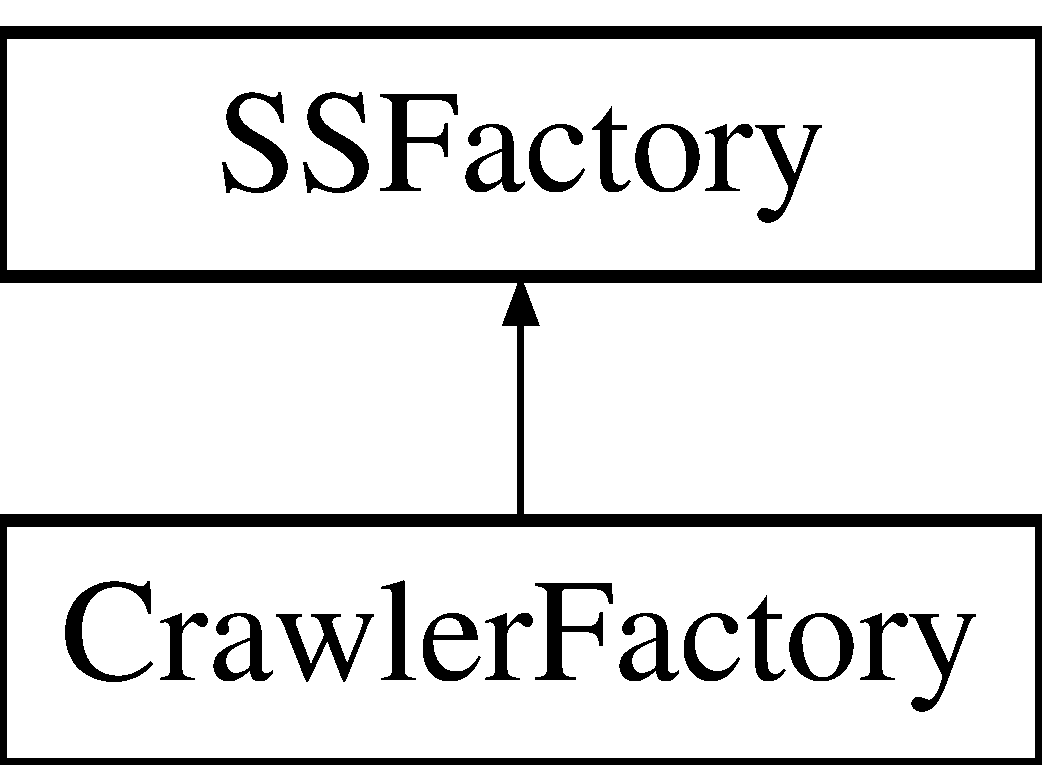
\includegraphics[height=2.000000cm]{classCrawlerFactory}
\end{center}
\end{figure}
\subsection*{Public Member Functions}
\begin{DoxyCompactItemize}
\item 
\hyperlink{classCrawlerFactory_ac99d39a8262df1890882edc33161a551}{Crawler\-Factory} ()
\begin{DoxyCompactList}\small\item\em Default constructor for factory. \end{DoxyCompactList}\end{DoxyCompactItemize}


\subsection{Detailed Description}
Factory class for constructing the state space for the crawler class. 

This class takes in a \hyperlink{classStateSpace}{State\-Space} pointer, and sets up the space for the crawler application. It arranges the state space into a 5x5 2\-D grid with the different joint configurations for each state. 

\subsection{Constructor \& Destructor Documentation}
\hypertarget{classCrawlerFactory_ac99d39a8262df1890882edc33161a551}{\index{Crawler\-Factory@{Crawler\-Factory}!Crawler\-Factory@{Crawler\-Factory}}
\index{Crawler\-Factory@{Crawler\-Factory}!CrawlerFactory@{Crawler\-Factory}}
\subsubsection[{Crawler\-Factory}]{\setlength{\rightskip}{0pt plus 5cm}Crawler\-Factory\-::\-Crawler\-Factory (
\begin{DoxyParamCaption}
{}
\end{DoxyParamCaption}
)}}\label{classCrawlerFactory_ac99d39a8262df1890882edc33161a551}


Default constructor for factory. 

$\ast$$\ast$$\ast$ Crawler Factory Class $\ast$$\ast$$\ast$///

Default constructor for factory. 

The documentation for this class was generated from the following files\-:\begin{DoxyCompactItemize}
\item 
crawler.\-h\item 
crawler.\-cpp\end{DoxyCompactItemize}

\hypertarget{classLidar}{\section{Lidar Class Reference}
\label{classLidar}\index{Lidar@{Lidar}}
}


\hyperlink{classLidar}{Lidar} class for reading distance values from \hyperlink{classLidar}{Lidar}.  




{\ttfamily \#include $<$crawler.\-h$>$}

\subsection*{Public Member Functions}
\begin{DoxyCompactItemize}
\item 
\hyperlink{classLidar_acc713b5eb35b95bee2ac4d5396b0fb5b}{Lidar} ()
\begin{DoxyCompactList}\small\item\em Default constructor. \end{DoxyCompactList}\item 
\hypertarget{classLidar_af1a22e6510e774e015f97e90dc8342a5}{void \hyperlink{classLidar_af1a22e6510e774e015f97e90dc8342a5}{read\-Sensor} ()}\label{classLidar_af1a22e6510e774e015f97e90dc8342a5}

\begin{DoxyCompactList}\small\item\em Grabs a distance reading from the \hyperlink{classLidar}{Lidar}. \end{DoxyCompactList}\item 
void \hyperlink{classLidar_a5d067f7656748755ea72ac31a9232ef5}{read\-Sensor\-N\-Times} (int n)
\begin{DoxyCompactList}\small\item\em Grabs N distance readings from the \hyperlink{classLidar}{Lidar} and saves their average. \end{DoxyCompactList}\item 
float \hyperlink{classLidar_a1085539adddae19ee6c3ce70ae4d7481}{get\-Voltage} ()
\begin{DoxyCompactList}\small\item\em Gets the voltage read from the most recent \hyperlink{classLidar}{Lidar} read. \end{DoxyCompactList}\item 
float \hyperlink{classLidar_ab8bb078d9dcff6162ce924fc6d0625d8}{get\-Distance} ()
\begin{DoxyCompactList}\small\item\em Gets the distance read from the most recent \hyperlink{classLidar}{Lidar} read. \end{DoxyCompactList}\end{DoxyCompactItemize}


\subsection{Detailed Description}
\hyperlink{classLidar}{Lidar} class for reading distance values from \hyperlink{classLidar}{Lidar}. 

This class is for reading the S\-F10/\-A Laser Altimeter for getting distance measurements to an object. 

\subsection{Constructor \& Destructor Documentation}
\hypertarget{classLidar_acc713b5eb35b95bee2ac4d5396b0fb5b}{\index{Lidar@{Lidar}!Lidar@{Lidar}}
\index{Lidar@{Lidar}!Lidar@{Lidar}}
\subsubsection[{Lidar}]{\setlength{\rightskip}{0pt plus 5cm}Lidar\-::\-Lidar (
\begin{DoxyParamCaption}
{}
\end{DoxyParamCaption}
)}}\label{classLidar_acc713b5eb35b95bee2ac4d5396b0fb5b}


Default constructor. 

$\ast$$\ast$$\ast$ \hyperlink{classLidar}{Lidar} Class $\ast$$\ast$$\ast$///

Default constructor 

\subsection{Member Function Documentation}
\hypertarget{classLidar_ab8bb078d9dcff6162ce924fc6d0625d8}{\index{Lidar@{Lidar}!get\-Distance@{get\-Distance}}
\index{get\-Distance@{get\-Distance}!Lidar@{Lidar}}
\subsubsection[{get\-Distance}]{\setlength{\rightskip}{0pt plus 5cm}float Lidar\-::get\-Distance (
\begin{DoxyParamCaption}
{}
\end{DoxyParamCaption}
)}}\label{classLidar_ab8bb078d9dcff6162ce924fc6d0625d8}


Gets the distance read from the most recent \hyperlink{classLidar}{Lidar} read. 

\begin{DoxyReturn}{Returns}
The distance read from the \hyperlink{classLidar}{Lidar} in meters. 
\end{DoxyReturn}
\hypertarget{classLidar_a1085539adddae19ee6c3ce70ae4d7481}{\index{Lidar@{Lidar}!get\-Voltage@{get\-Voltage}}
\index{get\-Voltage@{get\-Voltage}!Lidar@{Lidar}}
\subsubsection[{get\-Voltage}]{\setlength{\rightskip}{0pt plus 5cm}float Lidar\-::get\-Voltage (
\begin{DoxyParamCaption}
{}
\end{DoxyParamCaption}
)}}\label{classLidar_a1085539adddae19ee6c3ce70ae4d7481}


Gets the voltage read from the most recent \hyperlink{classLidar}{Lidar} read. 

\begin{DoxyReturn}{Returns}
The value the \hyperlink{classLidar}{Lidar} returned in volts. 
\end{DoxyReturn}
\hypertarget{classLidar_a5d067f7656748755ea72ac31a9232ef5}{\index{Lidar@{Lidar}!read\-Sensor\-N\-Times@{read\-Sensor\-N\-Times}}
\index{read\-Sensor\-N\-Times@{read\-Sensor\-N\-Times}!Lidar@{Lidar}}
\subsubsection[{read\-Sensor\-N\-Times}]{\setlength{\rightskip}{0pt plus 5cm}void Lidar\-::read\-Sensor\-N\-Times (
\begin{DoxyParamCaption}
\item[{int}]{n}
\end{DoxyParamCaption}
)}}\label{classLidar_a5d067f7656748755ea72ac31a9232ef5}


Grabs N distance readings from the \hyperlink{classLidar}{Lidar} and saves their average. 


\begin{DoxyParams}[1]{Parameters}
\mbox{\tt in}  & {\em n} & The number of readings to take. \\
\hline
\end{DoxyParams}


The documentation for this class was generated from the following files\-:\begin{DoxyCompactItemize}
\item 
crawler.\-h\item 
crawler.\-cpp\end{DoxyCompactItemize}

\hypertarget{classSSFactory}{\section{S\-S\-Factory Class Reference}
\label{classSSFactory}\index{S\-S\-Factory@{S\-S\-Factory}}
}


Factory class for constructing the state space for the application.  




{\ttfamily \#include $<$rl-\/lib\-\_\-state.\-h$>$}

Inheritance diagram for S\-S\-Factory\-:\begin{figure}[H]
\begin{center}
\leavevmode
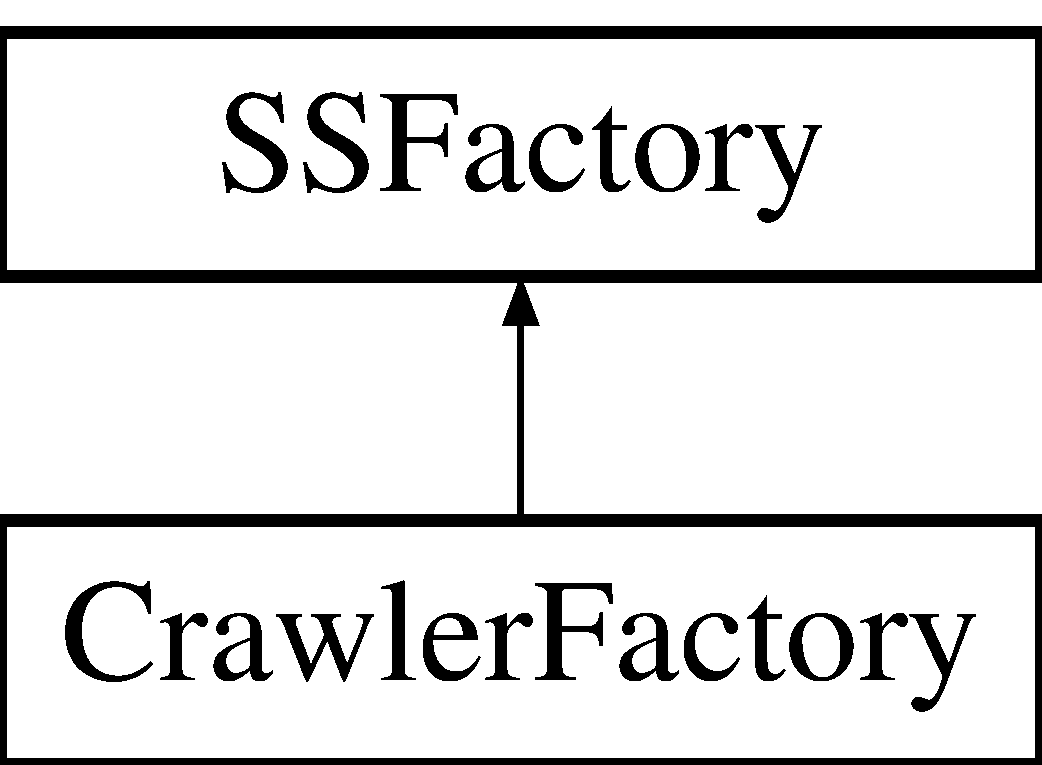
\includegraphics[height=2.000000cm]{classSSFactory}
\end{center}
\end{figure}
\subsection*{Public Member Functions}
\begin{DoxyCompactItemize}
\item 
\hyperlink{classSSFactory_a0e0861527997db2577d4aaf0ae27f039}{S\-S\-Factory} ()
\begin{DoxyCompactList}\small\item\em Default constructor for factory. \end{DoxyCompactList}\item 
void \hyperlink{classSSFactory_a07a9ec582bed0309dcc980e5fedddea8}{build\-State\-Space} ()
\begin{DoxyCompactList}\small\item\em Sets up the \hyperlink{classStateSpace}{State\-Space} object according to the crawler configuration. \end{DoxyCompactList}\item 
\hyperlink{classStateSpace}{State\-Space} $\ast$ \hyperlink{classSSFactory_a8a612db62fec0377b4f65465f58b91df}{get\-State\-Space} ()
\begin{DoxyCompactList}\small\item\em Produces the configured \hyperlink{classStateSpace}{State\-Space} object. \end{DoxyCompactList}\end{DoxyCompactItemize}


\subsection{Detailed Description}
Factory class for constructing the state space for the application. 

\subsection{Constructor \& Destructor Documentation}
\hypertarget{classSSFactory_a0e0861527997db2577d4aaf0ae27f039}{\index{S\-S\-Factory@{S\-S\-Factory}!S\-S\-Factory@{S\-S\-Factory}}
\index{S\-S\-Factory@{S\-S\-Factory}!SSFactory@{S\-S\-Factory}}
\subsubsection[{S\-S\-Factory}]{\setlength{\rightskip}{0pt plus 5cm}S\-S\-Factory\-::\-S\-S\-Factory (
\begin{DoxyParamCaption}
{}
\end{DoxyParamCaption}
)}}\label{classSSFactory_a0e0861527997db2577d4aaf0ae27f039}


Default constructor for factory. 

$\ast$$\ast$$\ast$ \hyperlink{classStateSpace}{State\-Space} Factory Class $\ast$$\ast$$\ast$///

Default constructor for factory. 

\subsection{Member Function Documentation}
\hypertarget{classSSFactory_a07a9ec582bed0309dcc980e5fedddea8}{\index{S\-S\-Factory@{S\-S\-Factory}!build\-State\-Space@{build\-State\-Space}}
\index{build\-State\-Space@{build\-State\-Space}!SSFactory@{S\-S\-Factory}}
\subsubsection[{build\-State\-Space}]{\setlength{\rightskip}{0pt plus 5cm}void S\-S\-Factory\-::build\-State\-Space (
\begin{DoxyParamCaption}
{}
\end{DoxyParamCaption}
)}}\label{classSSFactory_a07a9ec582bed0309dcc980e5fedddea8}


Sets up the \hyperlink{classStateSpace}{State\-Space} object according to the crawler configuration. 

Sets up the \hyperlink{classStateSpace}{State\-Space} object. \hypertarget{classSSFactory_a8a612db62fec0377b4f65465f58b91df}{\index{S\-S\-Factory@{S\-S\-Factory}!get\-State\-Space@{get\-State\-Space}}
\index{get\-State\-Space@{get\-State\-Space}!SSFactory@{S\-S\-Factory}}
\subsubsection[{get\-State\-Space}]{\setlength{\rightskip}{0pt plus 5cm}{\bf State\-Space} $\ast$ S\-S\-Factory\-::get\-State\-Space (
\begin{DoxyParamCaption}
{}
\end{DoxyParamCaption}
)}}\label{classSSFactory_a8a612db62fec0377b4f65465f58b91df}


Produces the configured \hyperlink{classStateSpace}{State\-Space} object. 

\begin{DoxyReturn}{Returns}
Returns the state space configured for the application.
\end{DoxyReturn}
Produces the configured \hyperlink{classStateSpace}{State\-Space} object. \begin{DoxyReturn}{Returns}
Returns the state space configured for the application. 
\end{DoxyReturn}


The documentation for this class was generated from the following files\-:\begin{DoxyCompactItemize}
\item 
rl-\/lib\-\_\-state.\-h\item 
rl-\/lib\-\_\-state.\-cpp\end{DoxyCompactItemize}

\hypertarget{classState}{\section{State Class Reference}
\label{classState}\index{State@{State}}
}


\hyperlink{classState}{State} class.  




{\ttfamily \#include $<$rl-\/lib\-\_\-state.\-h$>$}

\subsection*{Public Member Functions}
\begin{DoxyCompactItemize}
\item 
\hyperlink{classState_ab91bb1dd5aa6260ab2a456581daf9ec2}{State} ()
\begin{DoxyCompactList}\small\item\em Default constructor. \end{DoxyCompactList}\item 
\hyperlink{classState_acb29b7e6acb6ddac3bfe0629ef0e65b9}{State} (int n)
\begin{DoxyCompactList}\small\item\em Constructor for known action set size. \end{DoxyCompactList}\item 
\hyperlink{classState_a568030b37bd9340c190e2ca295f261d2}{State} (\hyperlink{classConfiguration}{Configuration} $\ast$state, \hyperlink{classConfigurationSet}{Configuration\-Set} $\ast$actions)
\begin{DoxyCompactList}\small\item\em Constructor with \hyperlink{classConfiguration}{Configuration} state and \hyperlink{classAction}{Action} set. \end{DoxyCompactList}\item 
\hypertarget{classState_afab438d92b90dc18d194dbd9c9c8bab3}{\hyperlink{classState_afab438d92b90dc18d194dbd9c9c8bab3}{$\sim$\-State} ()}\label{classState_afab438d92b90dc18d194dbd9c9c8bab3}

\begin{DoxyCompactList}\small\item\em Default destructor. \end{DoxyCompactList}\item 
void \hyperlink{classState_ab041e3de91fc35360d34c0e78c6d8543}{set\-Config} (\hyperlink{classConfiguration}{Configuration} $\ast$config)
\begin{DoxyCompactList}\small\item\em Set the state configuration. \end{DoxyCompactList}\item 
\hyperlink{classConfiguration}{Configuration} $\ast$ \hyperlink{classState_aa0472ec8cb28767154d4dd9eaac8a58d}{get\-Config} ()
\begin{DoxyCompactList}\small\item\em Method to get system configuration for this state. \end{DoxyCompactList}\item 
\hyperlink{classActionSet}{Action\-Set} $\ast$ \hyperlink{classState_a56deda372c59afd0d2b43e1211abffd4}{get\-Actions} ()
\begin{DoxyCompactList}\small\item\em Get the \hyperlink{classActionSet}{Action\-Set} for this \hyperlink{classState}{State}. \end{DoxyCompactList}\end{DoxyCompactItemize}


\subsection{Detailed Description}
\hyperlink{classState}{State} class. 

This class is for creating states that can be used with different Reinforcement Learning Algorithms. 

\subsection{Constructor \& Destructor Documentation}
\hypertarget{classState_ab91bb1dd5aa6260ab2a456581daf9ec2}{\index{State@{State}!State@{State}}
\index{State@{State}!State@{State}}
\subsubsection[{State}]{\setlength{\rightskip}{0pt plus 5cm}State\-::\-State (
\begin{DoxyParamCaption}
{}
\end{DoxyParamCaption}
)}}\label{classState_ab91bb1dd5aa6260ab2a456581daf9ec2}


Default constructor. 

$\ast$$\ast$$\ast$ \hyperlink{classState}{State} Class $\ast$$\ast$$\ast$/// \hypertarget{classState_acb29b7e6acb6ddac3bfe0629ef0e65b9}{\index{State@{State}!State@{State}}
\index{State@{State}!State@{State}}
\subsubsection[{State}]{\setlength{\rightskip}{0pt plus 5cm}State\-::\-State (
\begin{DoxyParamCaption}
\item[{int}]{n}
\end{DoxyParamCaption}
)}}\label{classState_acb29b7e6acb6ddac3bfe0629ef0e65b9}


Constructor for known action set size. 


\begin{DoxyParams}[1]{Parameters}
\mbox{\tt in}  & {\em n} & The number of actions for the state. \\
\hline
\end{DoxyParams}
\hypertarget{classState_a568030b37bd9340c190e2ca295f261d2}{\index{State@{State}!State@{State}}
\index{State@{State}!State@{State}}
\subsubsection[{State}]{\setlength{\rightskip}{0pt plus 5cm}State\-::\-State (
\begin{DoxyParamCaption}
\item[{{\bf Configuration} $\ast$}]{state, }
\item[{{\bf Configuration\-Set} $\ast$}]{actions}
\end{DoxyParamCaption}
)}}\label{classState_a568030b37bd9340c190e2ca295f261d2}


Constructor with \hyperlink{classConfiguration}{Configuration} state and \hyperlink{classAction}{Action} set. 


\begin{DoxyParams}[1]{Parameters}
\mbox{\tt in}  & {\em state} & The \hyperlink{classConfiguration}{Configuration} for that state. \\
\hline
\mbox{\tt in}  & {\em actions} & The \hyperlink{classConfigurationSet}{Configuration\-Set} describing the actions in that state. \\
\hline
\end{DoxyParams}


\subsection{Member Function Documentation}
\hypertarget{classState_a56deda372c59afd0d2b43e1211abffd4}{\index{State@{State}!get\-Actions@{get\-Actions}}
\index{get\-Actions@{get\-Actions}!State@{State}}
\subsubsection[{get\-Actions}]{\setlength{\rightskip}{0pt plus 5cm}{\bf Action\-Set}$\ast$ State\-::get\-Actions (
\begin{DoxyParamCaption}
{}
\end{DoxyParamCaption}
)}}\label{classState_a56deda372c59afd0d2b43e1211abffd4}


Get the \hyperlink{classActionSet}{Action\-Set} for this \hyperlink{classState}{State}. 

\begin{DoxyReturn}{Returns}
Pointer to the \hyperlink{classActionSet}{Action\-Set} that belongs to this \hyperlink{classState}{State}. 
\end{DoxyReturn}
\hypertarget{classState_aa0472ec8cb28767154d4dd9eaac8a58d}{\index{State@{State}!get\-Config@{get\-Config}}
\index{get\-Config@{get\-Config}!State@{State}}
\subsubsection[{get\-Config}]{\setlength{\rightskip}{0pt plus 5cm}{\bf Configuration} $\ast$ State\-::get\-Config (
\begin{DoxyParamCaption}
{}
\end{DoxyParamCaption}
)}}\label{classState_aa0472ec8cb28767154d4dd9eaac8a58d}


Method to get system configuration for this state. 

\begin{DoxyReturn}{Returns}
The \hyperlink{classConfiguration}{Configuration} of this state. 
\end{DoxyReturn}
\hypertarget{classState_ab041e3de91fc35360d34c0e78c6d8543}{\index{State@{State}!set\-Config@{set\-Config}}
\index{set\-Config@{set\-Config}!State@{State}}
\subsubsection[{set\-Config}]{\setlength{\rightskip}{0pt plus 5cm}void State\-::set\-Config (
\begin{DoxyParamCaption}
\item[{{\bf Configuration} $\ast$}]{config}
\end{DoxyParamCaption}
)}}\label{classState_ab041e3de91fc35360d34c0e78c6d8543}


Set the state configuration. 


\begin{DoxyParams}[1]{Parameters}
\mbox{\tt in}  & {\em config} & \hyperlink{classConfiguration}{Configuration} to set the \hyperlink{classState}{State} to. \\
\hline
\end{DoxyParams}


The documentation for this class was generated from the following files\-:\begin{DoxyCompactItemize}
\item 
rl-\/lib\-\_\-state.\-h\item 
rl-\/lib\-\_\-state.\-cpp\end{DoxyCompactItemize}

\hypertarget{classStateSpace}{\section{State\-Space Class Reference}
\label{classStateSpace}\index{State\-Space@{State\-Space}}
}


\hyperlink{classStateSpace}{State\-Space} class.  




{\ttfamily \#include $<$rl-\/lib\-\_\-state.\-h$>$}

\subsection*{Public Member Functions}
\begin{DoxyCompactItemize}
\item 
\hyperlink{classStateSpace_a9809804afcf94ebe347e19300d1a072e}{State\-Space} ()
\begin{DoxyCompactList}\small\item\em Default constructor. \end{DoxyCompactList}\item 
\hyperlink{classStateSpace_a432d9ee4a72d3f6da5f0d09f2656a8ae}{State\-Space} (int n)
\begin{DoxyCompactList}\small\item\em Constructor for known number of states. \end{DoxyCompactList}\item 
void \hyperlink{classStateSpace_a261398949f30aa06ad9c5ed4b2426cb1}{push} (\hyperlink{classState}{State} $\ast$s)
\begin{DoxyCompactList}\small\item\em Add \hyperlink{classState}{State} to the set. \end{DoxyCompactList}\item 
\hyperlink{classState}{State} $\ast$ \hyperlink{classStateSpace_add66f2ade4b11919338ed101241f281a}{pop} ()
\begin{DoxyCompactList}\small\item\em Remove \hyperlink{classState}{State} from the set. \end{DoxyCompactList}\item 
bool \hyperlink{classStateSpace_a0a4d75d9f92d513220743e8ca4621d65}{is\-Empty} ()
\begin{DoxyCompactList}\small\item\em Are there any objects in the set? \end{DoxyCompactList}\item 
int \hyperlink{classStateSpace_a531782c8f2e1fdffcfbd4127b383477f}{size} ()
\begin{DoxyCompactList}\small\item\em How many Configurations are in this set? \end{DoxyCompactList}\item 
\hypertarget{classStateSpace_aa93bb010b217aa918ac2f68758d51247}{\hyperlink{classStateSpaceIter}{State\-Space\-Iter} $\ast$ \hyperlink{classStateSpace_aa93bb010b217aa918ac2f68758d51247}{create\-Iter} () const }\label{classStateSpace_aa93bb010b217aa918ac2f68758d51247}

\begin{DoxyCompactList}\small\item\em Create iterator for set. \end{DoxyCompactList}\end{DoxyCompactItemize}
\subsection*{Friends}
\begin{DoxyCompactItemize}
\item 
\hypertarget{classStateSpace_a27384fd8b0bff77b9033cab49a33de0f}{class \hyperlink{classStateSpace_a27384fd8b0bff77b9033cab49a33de0f}{State\-Space\-Iter}}\label{classStateSpace_a27384fd8b0bff77b9033cab49a33de0f}

\begin{DoxyCompactList}\small\item\em Declare iterator class as friend. \end{DoxyCompactList}\end{DoxyCompactItemize}


\subsection{Detailed Description}
\hyperlink{classStateSpace}{State\-Space} class. 

This class is for \hyperlink{classState}{State} Spaces that can be used with different Reinforcement Learning Algorithms. 

\subsection{Constructor \& Destructor Documentation}
\hypertarget{classStateSpace_a9809804afcf94ebe347e19300d1a072e}{\index{State\-Space@{State\-Space}!State\-Space@{State\-Space}}
\index{State\-Space@{State\-Space}!StateSpace@{State\-Space}}
\subsubsection[{State\-Space}]{\setlength{\rightskip}{0pt plus 5cm}State\-Space\-::\-State\-Space (
\begin{DoxyParamCaption}
{}
\end{DoxyParamCaption}
)}}\label{classStateSpace_a9809804afcf94ebe347e19300d1a072e}


Default constructor. 

$\ast$$\ast$$\ast$ \hyperlink{classStateSpace}{State\-Space} Class $\ast$$\ast$$\ast$/// \hypertarget{classStateSpace_a432d9ee4a72d3f6da5f0d09f2656a8ae}{\index{State\-Space@{State\-Space}!State\-Space@{State\-Space}}
\index{State\-Space@{State\-Space}!StateSpace@{State\-Space}}
\subsubsection[{State\-Space}]{\setlength{\rightskip}{0pt plus 5cm}State\-Space\-::\-State\-Space (
\begin{DoxyParamCaption}
\item[{int}]{n}
\end{DoxyParamCaption}
)}}\label{classStateSpace_a432d9ee4a72d3f6da5f0d09f2656a8ae}


Constructor for known number of states. 


\begin{DoxyParams}[1]{Parameters}
\mbox{\tt in}  & {\em n} & Number of system states. \\
\hline
\end{DoxyParams}


\subsection{Member Function Documentation}
\hypertarget{classStateSpace_a0a4d75d9f92d513220743e8ca4621d65}{\index{State\-Space@{State\-Space}!is\-Empty@{is\-Empty}}
\index{is\-Empty@{is\-Empty}!StateSpace@{State\-Space}}
\subsubsection[{is\-Empty}]{\setlength{\rightskip}{0pt plus 5cm}bool State\-Space\-::is\-Empty (
\begin{DoxyParamCaption}
{}
\end{DoxyParamCaption}
)}}\label{classStateSpace_a0a4d75d9f92d513220743e8ca4621d65}


Are there any objects in the set? 

\begin{DoxyReturn}{Returns}
Returns true if there is anything in the set. 
\end{DoxyReturn}
\hypertarget{classStateSpace_add66f2ade4b11919338ed101241f281a}{\index{State\-Space@{State\-Space}!pop@{pop}}
\index{pop@{pop}!StateSpace@{State\-Space}}
\subsubsection[{pop}]{\setlength{\rightskip}{0pt plus 5cm}{\bf State} $\ast$ State\-Space\-::pop (
\begin{DoxyParamCaption}
{}
\end{DoxyParamCaption}
)}}\label{classStateSpace_add66f2ade4b11919338ed101241f281a}


Remove \hyperlink{classState}{State} from the set. 

\begin{DoxyReturn}{Returns}
Pointer to the \hyperlink{classState}{State} object removed from the set. 
\end{DoxyReturn}
\hypertarget{classStateSpace_a261398949f30aa06ad9c5ed4b2426cb1}{\index{State\-Space@{State\-Space}!push@{push}}
\index{push@{push}!StateSpace@{State\-Space}}
\subsubsection[{push}]{\setlength{\rightskip}{0pt plus 5cm}void State\-Space\-::push (
\begin{DoxyParamCaption}
\item[{{\bf State} $\ast$}]{s}
\end{DoxyParamCaption}
)}}\label{classStateSpace_a261398949f30aa06ad9c5ed4b2426cb1}


Add \hyperlink{classState}{State} to the set. 

Add \hyperlink{classState}{State} to the space.


\begin{DoxyParams}[1]{Parameters}
\mbox{\tt in}  & {\em s} & Pointer to the \hyperlink{classState}{State} to be added to the set. \\
\hline
\end{DoxyParams}
\hypertarget{classStateSpace_a531782c8f2e1fdffcfbd4127b383477f}{\index{State\-Space@{State\-Space}!size@{size}}
\index{size@{size}!StateSpace@{State\-Space}}
\subsubsection[{size}]{\setlength{\rightskip}{0pt plus 5cm}int State\-Space\-::size (
\begin{DoxyParamCaption}
{}
\end{DoxyParamCaption}
)}}\label{classStateSpace_a531782c8f2e1fdffcfbd4127b383477f}


How many Configurations are in this set? 

Returns the size of the space.

\begin{DoxyReturn}{Returns}
Returns the number of Configurations in the set.

The number of states in the space. 
\end{DoxyReturn}


The documentation for this class was generated from the following files\-:\begin{DoxyCompactItemize}
\item 
rl-\/lib\-\_\-state.\-h\item 
rl-\/lib\-\_\-state.\-cpp\end{DoxyCompactItemize}

\hypertarget{classStateSpaceIter}{\section{State\-Space\-Iter Class Reference}
\label{classStateSpaceIter}\index{State\-Space\-Iter@{State\-Space\-Iter}}
}


Iterator class for \hyperlink{classStateSpace}{State\-Space}.  




{\ttfamily \#include $<$rl-\/lib\-\_\-state.\-h$>$}

\subsection*{Public Member Functions}
\begin{DoxyCompactItemize}
\item 
\hyperlink{classStateSpaceIter_a89178bf983f058a0ca4f4eb85e3e36bc}{State\-Space\-Iter} (const \hyperlink{classStateSpace}{State\-Space} $\ast$ss)
\begin{DoxyCompactList}\small\item\em Constructor taking \hyperlink{classStateSpace}{State\-Space} associated with iterator. \end{DoxyCompactList}\item 
\hypertarget{classStateSpaceIter_a7a4fd2989777c4c9af8ca0a2c6dae4bf}{void \hyperlink{classStateSpaceIter_a7a4fd2989777c4c9af8ca0a2c6dae4bf}{first} ()}\label{classStateSpaceIter_a7a4fd2989777c4c9af8ca0a2c6dae4bf}

\begin{DoxyCompactList}\small\item\em Set the iterator to the first element of the set. \end{DoxyCompactList}\item 
\hypertarget{classStateSpaceIter_a76f8c81ce415f9d504f334f9ae764e78}{void \hyperlink{classStateSpaceIter_a76f8c81ce415f9d504f334f9ae764e78}{next} ()}\label{classStateSpaceIter_a76f8c81ce415f9d504f334f9ae764e78}

\begin{DoxyCompactList}\small\item\em Increment the iterator. \end{DoxyCompactList}\item 
\hypertarget{classStateSpaceIter_a35788e48888ea301fd5cdc6ad38b444c}{bool \hyperlink{classStateSpaceIter_a35788e48888ea301fd5cdc6ad38b444c}{is\-Done} ()}\label{classStateSpaceIter_a35788e48888ea301fd5cdc6ad38b444c}

\begin{DoxyCompactList}\small\item\em Check to see if we are at the last element. \end{DoxyCompactList}\item 
\hypertarget{classStateSpaceIter_a5abee0ac163bfd54bb10b417a4ce08e8}{\hyperlink{classState}{State} $\ast$ \hyperlink{classStateSpaceIter_a5abee0ac163bfd54bb10b417a4ce08e8}{operator$\ast$} ()}\label{classStateSpaceIter_a5abee0ac163bfd54bb10b417a4ce08e8}

\begin{DoxyCompactList}\small\item\em Dereference operator. \end{DoxyCompactList}\item 
\hypertarget{classStateSpaceIter_a6ff0ed559987a980dd009f9d04ca0a29}{\hyperlink{classState}{State} $\ast$$\ast$ \hyperlink{classStateSpaceIter_a6ff0ed559987a980dd009f9d04ca0a29}{operator-\/$>$} () const }\label{classStateSpaceIter_a6ff0ed559987a980dd009f9d04ca0a29}

\begin{DoxyCompactList}\small\item\em Arrow operator. \end{DoxyCompactList}\end{DoxyCompactItemize}


\subsection{Detailed Description}
Iterator class for \hyperlink{classStateSpace}{State\-Space}. 

\subsection{Constructor \& Destructor Documentation}
\hypertarget{classStateSpaceIter_a89178bf983f058a0ca4f4eb85e3e36bc}{\index{State\-Space\-Iter@{State\-Space\-Iter}!State\-Space\-Iter@{State\-Space\-Iter}}
\index{State\-Space\-Iter@{State\-Space\-Iter}!StateSpaceIter@{State\-Space\-Iter}}
\subsubsection[{State\-Space\-Iter}]{\setlength{\rightskip}{0pt plus 5cm}State\-Space\-Iter\-::\-State\-Space\-Iter (
\begin{DoxyParamCaption}
\item[{const {\bf State\-Space} $\ast$}]{ss}
\end{DoxyParamCaption}
)}}\label{classStateSpaceIter_a89178bf983f058a0ca4f4eb85e3e36bc}


Constructor taking \hyperlink{classStateSpace}{State\-Space} associated with iterator. 

$\ast$$\ast$$\ast$ Iterator class for \hyperlink{classStateSpace}{State\-Space}. $\ast$$\ast$$\ast$///


\begin{DoxyParams}[1]{Parameters}
\mbox{\tt in}  & {\em as} & Pointer to the \hyperlink{classStateSpace}{State\-Space} for this iterator.\\
\hline
\end{DoxyParams}
Constructor taking \hyperlink{classStateSpace}{State\-Space} associated with iterator. 
\begin{DoxyParams}[1]{Parameters}
\mbox{\tt in}  & {\em as} & Pointer to the \hyperlink{classStateSpace}{State\-Space} for this iterator. \\
\hline
\end{DoxyParams}


The documentation for this class was generated from the following files\-:\begin{DoxyCompactItemize}
\item 
rl-\/lib\-\_\-state.\-h\item 
rl-\/lib\-\_\-state.\-cpp\end{DoxyCompactItemize}

%--- End generated contents ---

% Index
\newpage
\phantomsection
\addcontentsline{toc}{chapter}{Index}
\printindex

\end{document}
